\documentclass[../PianoDiQualifica_v4.0.0.tex]{subfiles}

\begin{document}
\appendix
\section{Attività di verifica}\label{sec:verifica}
Di seguito sono descritte ed analizzate le attività di verifica svolte su tutti i documenti, che vengono consegnati nelle varie revisioni di avanzamento del progetto.

\subsection{Tracciamento dei test}

	\kpanic\ ha deciso di utilizzare l'applicativo \gl{Trender} per facilitare il tracciamento sia delle relazioni fra casi d'uso e requisiti, che quelle fra requisiti e classi.
	%\subsection{Tracciamento Test di Validazione-Requisiti}

	%\newpage
	%\subsection{Tracciamento Requisiti-Test di Validazione}

	\subsubsection{Tracciamento Test di Sistema-Requisiti}
	\begin{longtable}[c] { >{\centering\arraybackslash}p{3cm} >{\centering\arraybackslash}p{3cm}}
		\toprule
		\centerline{\textbf{ID test}} & \centerline{\textbf{Requisiti}} \\
			\midrule
			TSFF1 & RFF1 \\
			\addlinespace[0.3em]
			\midrule
			\addlinespace[0.3em]
			TSOF2 & ROF2 \\
			\addlinespace[0.3em]
			\midrule
			\addlinespace[0.3em]
			TSOV3 & ROF3 \\
			\addlinespace[0.3em]
			\midrule
			\addlinespace[0.3em]
			TSOF4 & ROF4 \\
			\addlinespace[0.3em]
			\midrule
			\addlinespace[0.3em]
			TSOF5 & ROF5 \\
			\addlinespace[0.3em]
			\midrule
			\addlinespace[0.3em]
			TSOF6 & ROF6 \\
			\addlinespace[0.3em]
			\midrule
			\addlinespace[0.3em]
			TSOF7 & ROF7 \\
			\addlinespace[0.3em]
			\midrule
			\addlinespace[0.3em]
			TSOF8 & ROF8 \\
			\addlinespace[0.3em]
			\midrule
			\addlinespace[0.3em]
			TSOF9 & ROF9 \\
			\addlinespace[0.3em]
			\midrule
			\addlinespace[0.3em]
			TSQ10 & RFF10 \\
			\addlinespace[0.3em]
			\midrule
			\addlinespace[0.3em]
			TSOF11 & ROF11 \\
			\addlinespace[0.3em]
			\midrule
			\addlinespace[0.3em]
			TSOF12 & ROF12 \\
			\addlinespace[0.3em]
			\midrule
			\addlinespace[0.3em]
			TSOF13 & ROF13 \\
			\addlinespace[0.3em]
			\midrule
			\addlinespace[0.3em]
			TSOF14 & ROF14 \\
			\addlinespace[0.3em]
			\midrule
			\addlinespace[0.3em]
			TSOF15 & ROF15 \\
			\addlinespace[0.3em]
			\midrule
			\addlinespace[0.3em]
			TSOF16 & ROF16 \\
			\addlinespace[0.3em]
			\midrule
			\addlinespace[0.3em]
			TSOF17 & ROF17 \\
			\addlinespace[0.3em]
			\midrule
			\addlinespace[0.3em]
			TSOF18 & ROF18 \\
			\addlinespace[0.3em]
			\midrule
			\addlinespace[0.3em]
			TSOF19 & ROF19 \\
			\addlinespace[0.3em]
			\midrule
			\addlinespace[0.3em]
			TSOF20 & ROF20 \\
			\addlinespace[0.3em]
			\midrule
			\addlinespace[0.3em]
			TSOF21 & ROF21 \\
			\addlinespace[0.3em]
			\midrule
			\addlinespace[0.3em]
			TSOF22 & ROF22 \\
			\addlinespace[0.3em]
			\midrule
			\addlinespace[0.3em]
			TSOF23 & ROF23 \\
			\addlinespace[0.3em]
			\midrule
			\addlinespace[0.3em]
			TSOF24 & ROF24 \\
			\addlinespace[0.3em]
			\midrule
			\addlinespace[0.3em]
			TSOF25 & ROF25 \\
			\addlinespace[0.3em]
			\midrule
			\addlinespace[0.3em]
			TSOF26 & ROF26 \\
			\addlinespace[0.3em]
			\midrule
			\addlinespace[0.3em]
			TSOF27 & ROF27 \\
			\addlinespace[0.3em]
			\midrule
			\addlinespace[0.3em]
			TSFF28 & RFF28 \\
			\addlinespace[0.3em]
			\midrule
			\addlinespace[0.3em]
			TSOF29 & ROF29 \\
			\addlinespace[0.3em]
			\midrule
			\addlinespace[0.3em]
			TSOF30 & ROF30 \\
			\addlinespace[0.3em]
			\midrule
			\addlinespace[0.3em]
			TSQF31 & RFF31 \\
			\addlinespace[0.3em]
			\midrule
			\addlinespace[0.3em]
			TSOF32 & ROF32 \\
			\addlinespace[0.3em]
			\midrule
			\addlinespace[0.3em]
			TSOF33 & ROF33 \\
			\addlinespace[0.3em]
			\midrule
			\addlinespace[0.3em]
			TSOF34 & ROF34 \\
			\addlinespace[0.3em]
			\midrule
			\addlinespace[0.3em]
			TSOF35 & ROF35 \\
			\addlinespace[0.3em]
			\midrule
			\addlinespace[0.3em]
			TSOF36 & ROF36 \\
			\addlinespace[0.3em]
			\midrule
			\addlinespace[0.3em]
			TSOF37 & ROF37 \\
			\addlinespace[0.3em]
			\midrule
			\addlinespace[0.3em]
			TSOF38 & ROF38 \\
			\addlinespace[0.3em]
			\midrule
			\addlinespace[0.3em]
			TSOF39 & ROF39 \\
			\addlinespace[0.3em]
			\midrule
			\addlinespace[0.3em]
			TSOF40 & ROF40 \\
			\addlinespace[0.3em]
			\midrule
			\addlinespace[0.3em]
			TSOF41 & ROF41 \\
			\addlinespace[0.3em]
			\midrule
			\addlinespace[0.3em]
			TSOF42 & ROF42 \\
			\addlinespace[0.3em]
			\midrule
			\addlinespace[0.3em]
			TSQF43 & ROF43 \\
			\addlinespace[0.3em]
			\midrule
			\addlinespace[0.3em]
			TSOF44 & ROF44 \\
			\addlinespace[0.3em]
			\midrule
			\addlinespace[0.3em]
			TSOF45 & ROF45 \\
			\addlinespace[0.3em]
			\midrule
			\addlinespace[0.3em]
			TSOF46 & ROF46 \\
			\addlinespace[0.3em]
			\midrule
			\addlinespace[0.3em]
			TSOF47 & ROF47 \\
			\addlinespace[0.3em]
			\midrule
			\addlinespace[0.3em]
			TSOF48 & ROF48 \\
			\addlinespace[0.3em]
			\midrule
			\addlinespace[0.3em]
			TSOF49 & ROF49 \\
			\addlinespace[0.3em]
			\midrule
			\addlinespace[0.3em]
			TSOF50 & ROF50 \\
			\addlinespace[0.3em]
			\midrule
			\addlinespace[0.3em]
			TSOF51 & ROF51 \\
			\addlinespace[0.3em]
			\midrule
			\addlinespace[0.3em]
			TSOF52 & ROF52 \\
			\addlinespace[0.3em]
			\midrule
			\addlinespace[0.3em]
			TSOF53 & ROF53 \\
			\addlinespace[0.3em]
			\midrule
			\addlinespace[0.3em]
			TSOF54 & ROF54 \\
			\addlinespace[0.3em]
			\midrule
			\addlinespace[0.3em]
			TSOF55 & ROF55 \\
			\addlinespace[0.3em]
			\midrule
			\addlinespace[0.3em]
			TSOF56 & ROF56 \\
			\addlinespace[0.3em]
			\midrule
			\addlinespace[0.3em]
			TSOF57 & ROF57 \\
			\addlinespace[0.3em]
			\midrule
			\addlinespace[0.3em]
			TSOF58 & ROF58 \\
			\addlinespace[0.3em]
			\midrule
			\addlinespace[0.3em]
			TSOF59 & ROF59 \\
			\addlinespace[0.3em]
			\midrule
			\addlinespace[0.3em]
			TSOF60 & ROF60 \\
			\addlinespace[0.3em]
			\midrule
			\addlinespace[0.3em]
			TSOF61 & ROF61 \\
			\addlinespace[0.3em]
			\midrule
			\addlinespace[0.3em]
			TSOF62 & ROF62 \\
			\addlinespace[0.3em]
			\midrule
			\addlinespace[0.3em]
			TSOF63 & ROF63 \\
			\addlinespace[0.3em]
			\midrule
			\addlinespace[0.3em]
			TSOF64 & ROF64 \\
			\addlinespace[0.3em]
			\midrule
			\addlinespace[0.3em]
			TSOF65 & ROF65 \\
			\addlinespace[0.3em]
			\midrule
			\addlinespace[0.3em]
			TSOF66 & ROF66 \\
			\addlinespace[0.3em]
			\midrule
			\addlinespace[0.3em]
			TSOF67 & ROF67 \\
			\addlinespace[0.3em]
			\midrule
			\addlinespace[0.3em]
			TSOF68 & ROF68 \\
			\addlinespace[0.3em]
			\midrule
			\addlinespace[0.3em]
			TSOF69 & ROF69 \\
			\addlinespace[0.3em]
			\midrule
			\addlinespace[0.3em]
			TSOF70 & ROF70 \\
			\addlinespace[0.3em]
			\midrule
			\addlinespace[0.3em]
			TSOF71 & ROF71 \\
			\addlinespace[0.3em]
			\midrule
			\addlinespace[0.3em]
			TSOF72 & ROF72 \\
			\addlinespace[0.3em]
			\midrule
			\addlinespace[0.3em]
			TSOF73 & ROF73 \\
			\addlinespace[0.3em]
			\midrule
			\addlinespace[0.3em]
			TSOF74 & ROF74 \\
			\addlinespace[0.3em]
			\midrule
			\addlinespace[0.3em]
			TSOF76 & ROF76 \\
			\addlinespace[0.3em]
			\midrule
			\addlinespace[0.3em]
			TSOF78 & ROF78 \\
			\addlinespace[0.3em]
			\midrule
			\addlinespace[0.3em]
			TSOF79 & ROF79 \\
			\addlinespace[0.3em]
			\midrule
			\addlinespace[0.3em]
			TSOF80 & ROF80 \\
			\addlinespace[0.3em]
			\midrule
			\addlinespace[0.3em]
			TSOF81 & ROF81 \\
			\addlinespace[0.3em]
			\midrule
			\addlinespace[0.3em]
			TSOF82 & ROF82 \\
			\addlinespace[0.3em]
			\midrule
			\addlinespace[0.3em]
			TSOF83 & ROF83 \\
			\addlinespace[0.3em]
			\midrule
			\addlinespace[0.3em]
			TSOF84 & ROF84\\
			\addlinespace[0.3em]
			\midrule
			\addlinespace[0.3em]
			TSOF85 & ROF85 \\
			\addlinespace[0.3em]
			\midrule
			\addlinespace[0.3em]
			TSOF86 & ROF86 \\
			\addlinespace[0.3em]
			\midrule
			\addlinespace[0.3em]
			TSOF87 & ROF87 \\
			\addlinespace[0.3em]
			\midrule
			\addlinespace[0.3em]
			TSOF88 & ROF88 \\
			\addlinespace[0.3em]
			\midrule
			\addlinespace[0.3em]
			TSOF89 & ROF89\\
			\addlinespace[0.3em]
			\midrule
			\addlinespace[0.3em]
			TSOF90 & ROF90 \\
			\addlinespace[0.3em]
			\midrule
			\addlinespace[0.3em]
			TSOF91 & ROF91 \\
			\addlinespace[0.3em]
			\midrule
			\addlinespace[0.3em]
			TSOF92 & ROF92 \\
			\addlinespace[0.3em]
			\midrule
			\addlinespace[0.3em]
			TSOF93 & ROF93 \\
			\addlinespace[0.3em]
			\midrule
			\addlinespace[0.3em]
			TSOF94 & ROF94 \\
			\bottomrule
			\caption{Tracciamento Test di Sistema-Requisiti}
	\end{longtable}

	\subsubsection{Tracciamento Requisiti-Test di Sistema}
	\begin{longtable}[c] { >{\centering\arraybackslash}p{3cm} >{\centering\arraybackslash}p{3cm}}
		\toprule
		\centerline{\textbf{Requisiti}} & \centerline{\textbf{ID test}} \\
			\midrule
			RFF1 & TSFF1 \\
			\addlinespace[0.3em]
			\midrule
			\addlinespace[0.3em]
			ROF2 & TSOF2 \\
			\addlinespace[0.3em]
			\midrule
			\addlinespace[0.3em]
			ROF3 & TSOV3 \\
			\addlinespace[0.3em]
			\midrule
			\addlinespace[0.3em]
			ROF4 & TSOF4 \\
			\addlinespace[0.3em]
			\midrule
			\addlinespace[0.3em]
			ROF5 & TSOF5 \\
			\addlinespace[0.3em]
			\midrule
			\addlinespace[0.3em]
			ROF6 & TSOF6 \\
			\addlinespace[0.3em]
			\midrule
			\addlinespace[0.3em]
			ROF7 & TSOF7 \\
			\addlinespace[0.3em]
			\midrule
			\addlinespace[0.3em]
			ROF8 & TSOF8 \\
			\addlinespace[0.3em]
			\midrule
			\addlinespace[0.3em]
			ROF9 & TSOF9 \\
			\addlinespace[0.3em]
			\midrule
			\addlinespace[0.3em]
			RFF10 & TS2F10 \\
			\addlinespace[0.3em]
			\midrule
			\addlinespace[0.3em]
			ROF11 & TSOF11 \\
			\addlinespace[0.3em]
			\midrule
			\addlinespace[0.3em]
			ROF12 & TSOF12 \\
			\addlinespace[0.3em]
			\midrule
			\addlinespace[0.3em]
			ROF13 & TSOF13 \\
			\addlinespace[0.3em]
			\midrule
			\addlinespace[0.3em]
			ROF14 & TSOF14 \\
			\addlinespace[0.3em]
			\midrule
			\addlinespace[0.3em]
			ROF15 & TSOF15 \\
			\addlinespace[0.3em]
			\midrule
			\addlinespace[0.3em]
			ROF16 & TSOF16 \\
			\addlinespace[0.3em]
			\midrule
			\addlinespace[0.3em]
			ROF17 & TSOF17 \\
			\addlinespace[0.3em]
			\midrule
			\addlinespace[0.3em]
			ROF18 & TSOF18 \\
			\addlinespace[0.3em]
			\midrule
			\addlinespace[0.3em]
			ROF19 & TSOF19 \\
			\addlinespace[0.3em]
			\midrule
			\addlinespace[0.3em]
			ROF20 & TSOF20 \\
			\addlinespace[0.3em]
			\midrule
			\addlinespace[0.3em]
			ROF21 & TSOF21 \\
			\addlinespace[0.3em]
			\midrule
			\addlinespace[0.3em]
			ROF22 & TSOF22 \\
			\addlinespace[0.3em]
			\midrule
			\addlinespace[0.3em]
			ROF23 & TSOF23 \\
			\addlinespace[0.3em]
			\midrule
			\addlinespace[0.3em]
			ROF24 & TSOF24 \\
			\addlinespace[0.3em]
			\midrule
			\addlinespace[0.3em]
			ROF25 & TSOF25 \\
			\addlinespace[0.3em]
			\midrule
			\addlinespace[0.3em]
			ROF26 & TSOF26 \\
			\addlinespace[0.3em]
			\midrule
			\addlinespace[0.3em]
			ROF27 & TSOF27 \\
			\addlinespace[0.3em]
			\midrule
			\addlinespace[0.3em]
			RFF28 & TS2F28 \\
			\addlinespace[0.3em]
			\midrule
			\addlinespace[0.3em]
			ROF29 & TSOF29 \\
			\addlinespace[0.3em]
			\midrule
			\addlinespace[0.3em]
			ROF30 & TSOF30 \\
			\addlinespace[0.3em]
			\midrule
			\addlinespace[0.3em]
			RFF31 & TS2F31 \\
			\addlinespace[0.3em]
			\midrule
			\addlinespace[0.3em]
			ROF32 & TSOF32 \\
			\addlinespace[0.3em]
			\midrule
			\addlinespace[0.3em]
			ROF33 & TSOF33 \\
			\addlinespace[0.3em]
			\midrule
			\addlinespace[0.3em]
			ROF34 & TSOF34 \\
			\addlinespace[0.3em]
			\midrule
			\addlinespace[0.3em]
			ROF35 & TSOF35 \\
			\addlinespace[0.3em]
			\midrule
			\addlinespace[0.3em]
			ROF36 & TSOF36 \\
			\addlinespace[0.3em]
			\midrule
			\addlinespace[0.3em]
			ROF37 & TSOF37 \\
			\addlinespace[0.3em]
			\midrule
			\addlinespace[0.3em]
			ROF38 & TSOF38 \\
			\addlinespace[0.3em]
			\midrule
			\addlinespace[0.3em]
			ROF39 & TSOF39 \\
			\addlinespace[0.3em]
			\midrule
			\addlinespace[0.3em]
			ROF40 & TSOF40 \\
			\addlinespace[0.3em]
			\midrule
			\addlinespace[0.3em]
			ROF41 & TSOF41 \\
			\addlinespace[0.3em]
			\midrule
			\addlinespace[0.3em]
			ROF42 & TSOF42 \\
			\addlinespace[0.3em]
			\midrule
			\addlinespace[0.3em]
			ROF43 & TSQF43 \\
			\addlinespace[0.3em]
			\midrule
			\addlinespace[0.3em]
			ROF44 & TSOF44 \\
			\addlinespace[0.3em]
			\midrule
			\addlinespace[0.3em]
			ROF45 & TSOF45 \\
			\addlinespace[0.3em]
			\midrule
			\addlinespace[0.3em]
			ROF46 & TSOF46 \\
			\addlinespace[0.3em]
			\midrule
			\addlinespace[0.3em]
			ROF47 & TSOF47 \\
			\addlinespace[0.3em]
			\midrule
			\addlinespace[0.3em]
			ROF48 & TSOF48 \\
			\addlinespace[0.3em]
			\midrule
			\addlinespace[0.3em]
			ROF49 & TSOF49 \\
			\addlinespace[0.3em]
			\midrule
			\addlinespace[0.3em]
			ROF50 & TSOF50 \\
			\addlinespace[0.3em]
			\midrule
			\addlinespace[0.3em]
			ROF51 & TSOF51 \\
			\addlinespace[0.3em]
			\midrule
			\addlinespace[0.3em]
			ROF52 & TSOF52 \\
			\addlinespace[0.3em]
			\midrule
			\addlinespace[0.3em]
			ROF53 & TSOF53 \\
			\addlinespace[0.3em]
			\midrule
			\addlinespace[0.3em]
			ROF54 & TSOF54 \\
			\addlinespace[0.3em]
			\midrule
			\addlinespace[0.3em]
			ROF55 & TSOF55 \\
			\addlinespace[0.3em]
			\midrule
			\addlinespace[0.3em]
			ROF56 & TSOF56 \\
			\addlinespace[0.3em]
			\midrule
			\addlinespace[0.3em]
			ROF57 & TSOF57 \\
			\addlinespace[0.3em]
			\midrule
			\addlinespace[0.3em]
			ROF58 & TSOF58 \\
			\addlinespace[0.3em]
			\midrule
			\addlinespace[0.3em]
			ROF59 & TSOF59 \\
			\addlinespace[0.3em]
			\midrule
			\addlinespace[0.3em]
			ROF60 & TSOF60 \\
			\addlinespace[0.3em]
			\midrule
			\addlinespace[0.3em]
			ROF61 & TSOF61 \\
			\addlinespace[0.3em]
			\midrule
			\addlinespace[0.3em]
			ROF62 & TSOF62 \\
			\addlinespace[0.3em]
			\midrule
			\addlinespace[0.3em]
			ROF63 & TSOF63 \\
			\addlinespace[0.3em]
			\midrule
			\addlinespace[0.3em]
			ROF64 & TSOF64 \\
			\addlinespace[0.3em]
			\midrule
			\addlinespace[0.3em]
			ROF65 & TSOF65 \\
			\addlinespace[0.3em]
			\midrule
			\addlinespace[0.3em]
			ROF66 & TSOF66 \\
			\addlinespace[0.3em]
			\midrule
			\addlinespace[0.3em]
			ROF67 & TSOF67 \\
			\addlinespace[0.3em]
			\midrule
			\addlinespace[0.3em]
			ROF68 & TSOF68 \\
			\addlinespace[0.3em]
			\midrule
			\addlinespace[0.3em]
			ROF69 & TSOF69 \\
			\addlinespace[0.3em]
			\midrule
			\addlinespace[0.3em]
			ROF70 & TSOF70 \\
			\addlinespace[0.3em]
			\midrule
			\addlinespace[0.3em]
			ROF71 & TSOF71 \\
			\addlinespace[0.3em]
			\midrule
			\addlinespace[0.3em]
			ROF72 & TSOF72 \\
			\addlinespace[0.3em]
			\midrule
			\addlinespace[0.3em]
			ROF73 & TSOF73 \\
			\addlinespace[0.3em]
			\midrule
			\addlinespace[0.3em]
			ROF74 & TSOF74 \\
			\addlinespace[0.3em]
			\midrule
			\addlinespace[0.3em]
			ROF75 & TSOF75 \\
			\addlinespace[0.3em]
			\midrule
			\addlinespace[0.3em]
			ROF76 & TSOF76 \\
			\addlinespace[0.3em]
			\midrule
			\addlinespace[0.3em]
			ROF77 & TSOF77 \\
			\addlinespace[0.3em]
			\midrule
			\addlinespace[0.3em]
			ROF78 & TSOF78 \\
			\addlinespace[0.3em]
			\midrule
			\addlinespace[0.3em]
			ROF79 & TSOF79 \\
			\addlinespace[0.3em]
			\midrule
			\addlinespace[0.3em]
			ROF80 & TSOF80 \\
			\addlinespace[0.3em]
			\midrule
			\addlinespace[0.3em]
			ROF81 & TSOF81 \\
			\addlinespace[0.3em]
			\midrule
			\addlinespace[0.3em]
			ROF82 & TSOF82 \\
			\addlinespace[0.3em]
			\midrule
			\addlinespace[0.3em]
			ROF83 & TSOF83 \\
			\addlinespace[0.3em]
			\midrule
			\addlinespace[0.3em]
			ROF84 & TSOF84 \\
			\addlinespace[0.3em]
			\midrule
			\addlinespace[0.3em]
			ROF85 & TSOF85 \\
			\addlinespace[0.3em]
			\midrule
			\addlinespace[0.3em]
			ROF86 & TSOF86 \\
			\addlinespace[0.3em]
			\midrule
			\addlinespace[0.3em]
			ROF87 & TSOF87 \\
			\addlinespace[0.3em]
			\midrule
			\addlinespace[0.3em]
			ROF88 & TSOF88 \\
			\addlinespace[0.3em]
			\midrule
			\addlinespace[0.3em]
			ROF89 & TSOF89 \\
			\addlinespace[0.3em]
			\midrule
			\addlinespace[0.3em]
			ROF90 & TSOF90 \\
			\addlinespace[0.3em]
			\midrule
			\addlinespace[0.3em]
			ROF91 & TSOF91 \\
			\addlinespace[0.3em]
			\midrule
			\addlinespace[0.3em]
			ROF92 & TSOF92 \\
			\addlinespace[0.3em]
			\midrule
			\addlinespace[0.3em]
			ROF93 & TSOF93 \\
			\addlinespace[0.3em]
			\midrule
			\addlinespace[0.3em]
			ROF94 & TSOF94 \\
			\bottomrule
			\caption{Tracciamento Requisiti-Test di Sistema}
	\end{longtable}

	\newpage
	\subsubsection{Tracciamento Test di Integrazione-Componenti}
	Visto che l'architettura non prevede dei package che contengano esclusivamente View e Controller, essi sono stati inseriti nei package dei singoli componenti. Quando dovranno essere indicati per un test si userà il simbolo * per indicare il nome del package. Ad esempio nel package Login presente dentro AdministrationView nel Front-End per indicare la View si scriverà: *::*View, dove * indica il nome Login.
	\begin{longtable}[c] { >{\centering\arraybackslash}p{2cm} >{\centering\arraybackslash}p{11cm}}
		\toprule
		\centerline{\textbf{ID test}} & \centerline{\textbf{Componenti}} \\
			\midrule
			TI1 & Front-End \\
			\addlinespace[0.3em]
			\midrule
			\addlinespace[0.3em]
			TI2 & Back-End::Service \\
			\addlinespace[0.3em]
			\midrule
			\addlinespace[0.3em]
			TI3 & Front-End::GuestPage:GuestComponents::*::*View \\
			\addlinespace[0.3em]
			\midrule
			\addlinespace[0.3em]
			TI4 & Front-End::AdminPage::AdminComponents::*::*View \\
			\addlinespace[0.3em]
			\midrule
			\addlinespace[0.3em]
			TI5 & Models \\
			\addlinespace[0.3em]
			\midrule
			\addlinespace[0.3em]
			TI6 & Back-End \\
			\addlinespace[0.3em]
			\midrule
			\addlinespace[0.3em]
			TI7 & Back-End::Slack \\
			\addlinespace[0.3em]
			\midrule
			\addlinespace[0.3em]
			TI8 & Back-End::DatabaseInteraction \\
			\addlinespace[0.3em]
			\midrule
			\addlinespace[0.3em]
			TI9 & APIGateway (Front-End)\\
			\addlinespace[0.3em]
			\midrule
			\addlinespace[0.3em]
			TI10 & APIGateway (Back-End) \\
			\addlinespace[0.3em]
			\midrule
			\addlinespace[0.3em]
			TI11 &  Front-End::AdminPage::AdminComponents::*::*Controller \\
			\addlinespace[0.3em]
			\midrule
			\addlinespace[0.3em]
			TI12 & Front-End::GuestPage:GuestComponents::*::*Controller \\
			\addlinespace[0.3em]
			\midrule
			\addlinespace[0.3em]
			TI13 & Back-End::Interaction \\
			\addlinespace[0.3em]
			\midrule
			\addlinespace[0.3em]
			TI14 & Front-End::AdminPage::AdminServices \\
			\addlinespace[0.3em]
			\midrule
			\addlinespace[0.3em]
			TI15 & Front-End::GuestPage::GuestServices \\
			\addlinespace[0.3em]
			\midrule
			\addlinespace[0.3em]
			TI16 & Angular \\
			\addlinespace[0.3em]
			\midrule
			\addlinespace[0.3em]
			TI17 & ManageAuth \\
			\addlinespace[0.3em]
			\midrule
			\addlinespace[0.3em]
			TI18 & ManageSlack \\
			\addlinespace[0.3em]
			\midrule
			\addlinespace[0.3em]
			TI19 & ManageQuestion \\
			\addlinespace[0.3em]
			\midrule
			\addlinespace[0.3em]
			TI20 & ManageAdmin \\
			\addlinespace[0.3em]
			\midrule
			\addlinespace[0.3em]
			TI21 & ManageFirms \\
			\bottomrule
			\caption{Tracciamento Test di Integrazione-Componenti}
	\end{longtable}

	\newpage
	\subsubsection{Tracciamento Componenti-Test di Integrazione}
	Dato che l'architettura non prevede dei package che contengano esclusivamente View e Controller, essi sono stati inseriti nei package dei singoli componenti. Quando dovranno essere indicati per un test si userà il simbolo * per indicare il nome del package. Ad esempio nel package Login presente dentro AdministrationView nel Front-End per indicare la View si scriverà: *::*View, dove * indica il nome Login.
	\begin{longtable}[c] { >{\centering\arraybackslash}p{11cm} >{\centering\arraybackslash}p{2cm}}
		\toprule
		\centerline{\textbf{Componenti}} & \centerline{\textbf{ID test}} \\
			\midrule
			Front-End & TI1 \\
			\addlinespace[0.3em]
			\midrule
			\addlinespace[0.3em]
			Back-End::Service & TI2 \\
			\addlinespace[0.3em]
			\midrule
			\addlinespace[0.3em]
			Front-End::GuestPage:GuestComponents::*::*View & TI3 \\
			\addlinespace[0.3em]
			\midrule
			\addlinespace[0.3em]
			Front-End::AdminPage::AdminComponents::*::*View & TI4\\
			\addlinespace[0.3em]
			\midrule
			\addlinespace[0.3em]
			Models & TI5\\
			\addlinespace[0.3em]
			\midrule
			\addlinespace[0.3em]
			Back-End & TI6\\
			\addlinespace[0.3em]
			\midrule
			\addlinespace[0.3em]
			Back-End::Slack & TI7\\
			\addlinespace[0.3em]
			\midrule
			\addlinespace[0.3em]
			Back-End::DatabaseInteraction & TI8 \\
			\addlinespace[0.3em]
			\midrule
			\addlinespace[0.3em]
			APIGateway (Front-End) & TI9\\
			\addlinespace[0.3em]
			\midrule
			\addlinespace[0.3em]
			APIGateway (Back-End) & TI10\\
			\addlinespace[0.3em]
			\midrule
			\addlinespace[0.3em]
			Front-End::AdminPage::AdminComponents::*::*Controller & TI11\\
			\addlinespace[0.3em]
			\midrule
			\addlinespace[0.3em]
			Front-End::GuestPage:GuestComponents::*::*Controller & TI12\\
			\addlinespace[0.3em]
			\midrule
			\addlinespace[0.3em]
			Back-End::Interaction & TI13 \\
			\addlinespace[0.3em]
			\midrule
			\addlinespace[0.3em]
			Front-End::AdminPage::AdminServices & TI14\\
			\addlinespace[0.3em]
			\midrule
			\addlinespace[0.3em]
			Front-End::GuestPage::GuestServices & TI15 \\
			\addlinespace[0.3em]
			\midrule
			\addlinespace[0.3em]
			Angular & TI16\\
			\addlinespace[0.3em]
			\midrule
			\addlinespace[0.3em]
			ManageAuth & TI17 \\
			\addlinespace[0.3em]
			\midrule
			\addlinespace[0.3em]
			ManageSlack & TI18 \\
			\addlinespace[0.3em]
			\midrule
			\addlinespace[0.3em]
			ManageQuestion & TI19 \\
			\addlinespace[0.3em]
			\midrule
			\addlinespace[0.3em]
			ManageAdmin & TI20 \\
			\addlinespace[0.3em]
			\midrule
			\addlinespace[0.3em]
			ManageFirms & TI21 \\
			\bottomrule
			\caption{Tracciamento Componenti-Test di Integrazione}
	\end{longtable}

	\newpage
	\subsubsection{Tracciamento Test di Unità-Metodi}
	\begin{longtable}[c] { >{\centering\arraybackslash}p{1,5cm} >{\centering\arraybackslash}p{13,5cm}}
		\toprule
		\centerline{\textbf{ID test}} & \centerline{\textbf{Metodo}}  \\
			\midrule
			TU0 & Back-End::Service::AdminService::addAdmin() \\
			\addlinespace[0.3em]
			\midrule
			\addlinespace[0.3em]
			TU1 & Back-End::Service::AdminService::updateAdmin() \\
			\addlinespace[0.3em]
			\midrule
			\addlinespace[0.3em]
			TU2 & Back-End::Service::AdminService::deleteAdmin() \\
			\addlinespace[0.3em]
			\midrule
			\addlinespace[0.3em]
			TU3 & Back-End::Service::AdminService::getAdmins() \\
			\addlinespace[0.3em]
			\midrule
			\addlinespace[0.3em]
			TU4 & Back-End::Service::AdminService::validateAdmin() \\
			\addlinespace[0.3em]
			\midrule
			\addlinespace[0.3em]
			TU5 & Back-End::Service::AdminService::validateUpdate() \\
			\addlinespace[0.3em]
			\midrule
			\addlinespace[0.3em]
			TU6 & Back-End::Service::AuthService::sendEmail() \\
			\addlinespace[0.3em]
			\midrule
			\addlinespace[0.3em]
			TU7 & Back-End::Service::AuthService::logout() \\
			\addlinespace[0.3em]
			\midrule
			\addlinespace[0.3em]
			TU8 & Back-End::Service::AuthService::login() \\
			\addlinespace[0.3em]
			\midrule
			\addlinespace[0.3em]
			TU9 & Back-End::Service::AuthService::verifyLogin() \\
			\addlinespace[0.3em]
			\midrule
			\addlinespace[0.3em]
			TU10 & Back-End::Service::AuthService::validateAuth() \\
			\addlinespace[0.3em]
			\midrule
			\addlinespace[0.3em]
			TU11 & Back-End::Service::AuthService::passwordRecoveryToken() \\
			\addlinespace[0.3em]
			\midrule
			\addlinespace[0.3em]
			TU12 & Back-End::Service::FirmService::getFirms() \\
			\addlinespace[0.3em]
			\midrule
			\addlinespace[0.3em]
			TU13 & Back-End::Service::FirmService::updateFirm() \\
			\addlinespace[0.3em]
			\midrule
			\addlinespace[0.3em]
			TU14 & Back-End::Service::FirmService::getGuestConversation() \\
			\addlinespace[0.3em]
			\midrule
			\addlinespace[0.3em]
			TU15 & Back-End::Service::FirmService::existFirm() \\
			\addlinespace[0.3em]
			\midrule
			\addlinespace[0.3em]
			TU16 & Back-End::Service::FirmService::existGuest() \\
			\addlinespace[0.3em]
			\midrule
			\addlinespace[0.3em]
			TU17 & Back-End::Service::FirmService::validateGuest() \\
			\addlinespace[0.3em]
			\midrule
			\addlinespace[0.3em]
			TU18 & Back-End::Service::FirmService::validateFirm() \\
			\addlinespace[0.3em]
			\midrule
			\addlinespace[0.3em]
			TU19 & Back-End::Service::SlackService::InfoSlack::addToDefault() \\
			\addlinespace[0.3em]
			\midrule
			\addlinespace[0.3em]
			TU20 & Back-End::Service::SlackService::InfoSlack::refreshInterlocutors() \\
			\addlinespace[0.3em]
			\midrule
			\addlinespace[0.3em]
			TU21 & Back-End::Service::SlackService::InfoSlack::removeToDefault() \\
			\addlinespace[0.3em]
			\midrule
			\addlinespace[0.3em]
			TU22 & Back-End::Service::SlackService::InfoSlack::getInterlocutors() \\
			\addlinespace[0.3em]
			\midrule
			\addlinespace[0.3em]
			TU23 & Back-End::Service::SlackService::InfoSlack::getDefaultInterlocutors() \\
			\addlinespace[0.3em]
			\midrule
			\addlinespace[0.3em]
			TU24 & Back-End::Service::SlackService::InfoSlack::validateInterlocutor() \\
			\addlinespace[0.3em]
			\midrule
			\addlinespace[0.3em]
			TU25 & Back-End::Service::SlackService::MessageSlack::sendMessageChannel() \\
			\addlinespace[0.3em]
			\midrule
			\addlinespace[0.3em]
			TU26 & Back-End::Service::SlackService::MessageSlack::sendMessageGeneral() \\
			\addlinespace[0.3em]
			\midrule
			\addlinespace[0.3em]
			TU27 & Back-End::Service::QuestionService::addQuestion() \\
			\addlinespace[0.3em]
			\midrule
			\addlinespace[0.3em]
			TU28 & Back-End::Service::QuestionService::deleteQuestion() \\
			\addlinespace[0.3em]
			\midrule
			\addlinespace[0.3em]
			TU29 & Back-End::Service::QuestionService::getQuestions() \\
			\addlinespace[0.3em]
			\midrule
			\addlinespace[0.3em]
			TU30 & Back-End::Service::QuestionService::updateQuestion() \\
			\addlinespace[0.3em]
			\midrule
			\addlinespace[0.3em]
			TU31 & Back-End::Service::QuestionService::getActions() \\
			\addlinespace[0.3em]
			\midrule
			\addlinespace[0.3em]
			TU32 & Back-End::Service::QuestionService::getNextQuestion() \\
			\addlinespace[0.3em]
			\midrule
			\addlinespace[0.3em]
			TU33 & Back-End::Service::QuestionService::getFirstquestion() \\
			\addlinespace[0.3em]
			\midrule
			\addlinespace[0.3em]
			TU34 & Back-End::Service::QuestionService::getLastAnswerText() \\
			\addlinespace[0.3em]
			\midrule
			\addlinespace[0.3em]
			TU35 & Back-End::Service::QuestionService::validateQuestion() \\
			\addlinespace[0.3em]
			\midrule
			\addlinespace[0.3em]
			TU36 & Back-End::Service::DatabaseInteraction::DatabaseInteraction::add(), Service::DatabaseInteraction::DatabaseInteraction::delete(), Service::DatabaseInteraction::DatabaseInteraction::read(), Service::DatabaseInteraction::DatabaseInteraction::update() \\
			\addlinespace[0.3em]
			\midrule
			\addlinespace[0.3em]
			TU37 & Back-End::Slack::createChannel::createChannel() \\
			\addlinespace[0.3em]
			\midrule
			\addlinespace[0.3em]
			TU38 & Back-End::Slack::invite::invite() \\
			\addlinespace[0.3em]
			\midrule
			\addlinespace[0.3em]
			TU39 & Back-End::Slack::setPurpose::setPurpose() \\
			\addlinespace[0.3em]
			\midrule
			\addlinespace[0.3em]
			TU40 & Back-End::Slack::userList::userList() \\
			\addlinespace[0.3em]
			\midrule
			\addlinespace[0.3em]
			TU41 & Back-End::Slack::postMessage::postMessage() \\
			\addlinespace[0.3em]
			\midrule
			\addlinespace[0.3em]
			TU42 & Back-End::Skill::LambdaSkill::FlowModule::FlowModule::routine() \\
			\addlinespace[0.3em]
			\midrule
			\addlinespace[0.3em]
			TU43 & Back-End::Skill::LambdaSkill::FlowModule::FlowModule::getLastQuestion() \\
			\addlinespace[0.3em]
			\midrule
			\addlinespace[0.3em]
			TU44 & Back-End::Skill::LambdaSkill::FlowModule::FlowModule::getFirstQuestion() \\
			\addlinespace[0.3em]
			\midrule
			\addlinespace[0.3em]
			TU45 & Back-End::Skill::LambdaSkill::FlowModule::FlowModule::matchPossibileAnswer() \\
			\addlinespace[0.3em]
			\midrule
			\addlinespace[0.3em]
			TU46 & Back-End::Skill::LambdaSkill::FlowModule::FlowModule::composeNextQuestion() \\
			\addlinespace[0.3em]
			\midrule
			\addlinespace[0.3em]
			TU47 & Back-End::Skill::LambdaSkill::FlowModule::FlowModule::callAction() \\
			\addlinespace[0.3em]
			\midrule
			\addlinespace[0.3em]
			TU48 & Back-End::Skill::LambdaSkill::FlowModule::FlowModule::logAnswerOnDB() \\
			\addlinespace[0.3em]
			\midrule
			\addlinespace[0.3em]
			TU49 & Front-End::AdminPage::AdminServices::ManageAdministratorsService::addAdmin(), AdminServices::ManageAdministratorsService::deleteAdmin(), AdminServices::ManageAdministratorsService::getAdmins(), AdminServices::ManageAdministratorsService::updateAdmin() \\
			\addlinespace[0.3em]
			\midrule
			\addlinespace[0.3em]
			TU50 & Front-End::AdminPage::AdminServices::ManageFirmsService::getFirms(), AdminServices::ManageFirmsService::getConvertions() \\
			\addlinespace[0.3em]
			\midrule
			\addlinespace[0.3em]
			TU51 & Front-End::AdminPage::AdminServices::ManageSlackService::setInterlocutorToDefault(), AdminServices::ManageSlackService::getDefaultInterlocutors(), AdminServices::ManageSlackService::getInterlocutors(), AdminServices::ManageSlackService::removeInterlocutorFromDefault(), AdminServices::ManageSlackService::updateInterlocutors() \\
			\addlinespace[0.3em]
			\midrule
			\addlinespace[0.3em]
			TU52 & Front-End::AdminPage::AdminServices::ManageQuestionsService::addQuestion(), AdminServices::ManageQuestionsService::deleteQuestion(), AdminServices::ManageQuestionsService::getQuestions() \\
			\addlinespace[0.3em]
			\midrule
			\addlinespace[0.3em]
			TU53 & Front-End::AdminPage::AdminServices::AuthService::login(), AdminServices::AuthService::update(), AdminServices::AuthService::logout(), AdminServices::AuthService::checkToken() \\
			\bottomrule
			\caption{Tracciamento Test di Unità-Metodi}
	\end{longtable}

	\newpage
	\subsubsection{Tracciamento Metodi-Test di Unità}
	\begin{longtable}[c] {>{\centering\arraybackslash}p{13,5cm} >{\centering\arraybackslash}p{1,5cm}}
		\toprule
		\centerline{\textbf{Metodo}} & \centerline{\textbf{ID test}}  \\
			\midrule
	 		Back-End::Service::AdminService::addAdmin() & TU0 \\
	 		\addlinespace[0.3em]
			\midrule
			\addlinespace[0.3em]
			Back-End::Service::AdminService::updateAdmin() & TU1 \\
			\addlinespace[0.3em]
			\midrule
			\addlinespace[0.3em]
 			Back-End::Service::AdminService::deleteAdmin() & TU2 \\
 			\addlinespace[0.3em]
			\midrule
			\addlinespace[0.3em]
 			Back-End::Service::AdminService::getAdmins() & TU3 \\
 			\addlinespace[0.3em]
			\midrule
			\addlinespace[0.3em]
			Back-End::Service::AdminService::validateAdmin() & TU4 \\
 			\addlinespace[0.3em]
			\midrule
			\addlinespace[0.3em]
 			Back-End::Service::AdminService::validateUpdate() & TU5 \\
 			\addlinespace[0.3em]
			\midrule
			\addlinespace[0.3em]
 			Back-End::Service::AuthService::sendEmail() & TU6 \\
 			\addlinespace[0.3em]
			\midrule
			\addlinespace[0.3em]
 			Back-End::Service::AuthService::logout() & TU7 \\
 			\addlinespace[0.3em]
			\midrule
			\addlinespace[0.3em]
 			Back-End::Service::AuthService::login() & TU8 \\
 			\addlinespace[0.3em]
			\midrule
			\addlinespace[0.3em]
			Back-End::Service::AuthService::verifyLogin() & TU9 \\
 			\addlinespace[0.3em]
			\midrule
			\addlinespace[0.3em]
			Back-End::Service::AuthService::validateAuth() & TU10 \\
 			\addlinespace[0.3em]
			\midrule
			\addlinespace[0.3em]
			Back-End::Service::AuthService::passwordRecoveryToken() & TU11 \\
 			\addlinespace[0.3em]
			\midrule
			\addlinespace[0.3em]
			Back-End::Service::FirmService::getFirms() & TU12 \\
 			\addlinespace[0.3em]
			\midrule
			\addlinespace[0.3em]
			Back-End::Service::FirmService::updateFirm() & TU13 \\
 			\addlinespace[0.3em]
			\midrule
			\addlinespace[0.3em]
 			Back-End::Service::FirmService::getGuestConversation() & TU14 \\
 			\addlinespace[0.3em]
			\midrule
			\addlinespace[0.3em]
			Back-End::Service::FirmService::existFirm() & TU15 \\
			\addlinespace[0.3em]
			\midrule
			\addlinespace[0.3em]
			Back-End::Service::FirmService::existGuest() & TU16 \\
 			\addlinespace[0.3em]
			\midrule
			\addlinespace[0.3em]
			Back-End::Service::FirmService::validateGuest() & TU17 \\
 			\addlinespace[0.3em]
			\midrule
			\addlinespace[0.3em]
 			Back-End::Service::FirmService::validateFirm() & TU18 \\
 			\addlinespace[0.3em]
			\midrule
			\addlinespace[0.3em]
 			Back-End::Service::SlackService::InfoSlack::addToDefault() & TU19 \\
 			\addlinespace[0.3em]
			\midrule
			\addlinespace[0.3em]
			Back-End::Service::SlackService::InfoSlack::refreshInterlocutors() & TU20 \\
			\addlinespace[0.3em]
			\midrule
			\addlinespace[0.3em]
 			Back-End::Service::SlackService::InfoSlack::removeToDefault() & TU21 \\
 			\addlinespace[0.3em]
			\midrule
			\addlinespace[0.3em]
			Back-End::Service::SlackService::InfoSlack::getInterlocutors() & TU22 \\
 			\addlinespace[0.3em]
			\midrule
			\addlinespace[0.3em]
 			Back-End::Service::SlackService::InfoSlack::getDefaultInterlocutors() & TU23 \\
 			\addlinespace[0.3em]
			\midrule
			\addlinespace[0.3em]
			Back-End::Service::SlackService::InfoSlack::validateInterlocutor() & TU24 \\
 			\addlinespace[0.3em]
			\midrule
			\addlinespace[0.3em]
			Back-End::Service::SlackService::MessageSlack::sendMessageChannel() & TU25 \\
 			\addlinespace[0.3em]
			\midrule
			\addlinespace[0.3em]
 			Back-End::Service::SlackService::MessageSlack::sendMessageGeneral() & TU26 \\
 			\addlinespace[0.3em]
			\midrule
			\addlinespace[0.3em]
 			Back-End::Service::QuestionService::addQuestion() & TU27 \\
 			\addlinespace[0.3em]
			\midrule
			\addlinespace[0.3em]
 			Back-End::Service::QuestionService::deleteQuestion() & TU28 \\
 			\addlinespace[0.3em]
			\midrule
			\addlinespace[0.3em]
 			Back-End::Service::QuestionService::getQuestions() & TU29 \\
 			\addlinespace[0.3em]
			\midrule
			\addlinespace[0.3em]
 			Back-End::Service::QuestionService::updateQuestion() & TU30 \\
 			\addlinespace[0.3em]
			\midrule
			\addlinespace[0.3em]
 			Back-End::Service::QuestionService::getActions() & TU31 \\
 			\addlinespace[0.3em]
			\midrule
			\addlinespace[0.3em]
			Back-End::Service::QuestionService::getNextQuestion() & TU32 \\
 			\addlinespace[0.3em]
			\midrule
			\addlinespace[0.3em]
 			Back-End::Service::QuestionService::getFirstquestion() & TU33 \\
 			\addlinespace[0.3em]
			\midrule
			\addlinespace[0.3em]
 			Back-End::Service::QuestionService::getLastAnswerText() & TU34\\
 			\addlinespace[0.3em]
			\midrule
			\addlinespace[0.3em]
			Back-End::Service::QuestionService::validateQuestion() & TU35 \\
 			\addlinespace[0.3em]
			\midrule
			\addlinespace[0.3em]
 			Back-End::Service::DatabaseInteraction::DatabaseInteraction::add() & TU36 \\
 			\addlinespace[0.3em]
			\midrule
			\addlinespace[0.3em]
			Back-End::Service::DatabaseInteraction::DatabaseInteraction::delete() & TU36 \\
 			\addlinespace[0.3em]
			\midrule
			\addlinespace[0.3em]
 			Back-End::Service::DatabaseInteraction::DatabaseInteraction::read() & TU36 \\
 			\addlinespace[0.3em]
			\midrule
			\addlinespace[0.3em]
 			Back-End::Service::DatabaseInteraction::DatabaseInteraction::update() & TU36 \\
			\addlinespace[0.3em]
			\midrule
			\addlinespace[0.3em]
 			Back-End::Slack::createChannel::createChannel() & TU37 \\
 			\addlinespace[0.3em]
			\midrule
			\addlinespace[0.3em]
 			Back-End::Slack::invite::invite() & TU38 \\
 			\addlinespace[0.3em]
			\midrule
			\addlinespace[0.3em]
 			Back-End::Slack::setPurpose::setPurpose() & TU39 \\
			\addlinespace[0.3em]
			\midrule
			\addlinespace[0.3em]
 			Back-End::Slack::userList::userList() & TU40 \\
 			\addlinespace[0.3em]
			\midrule
			\addlinespace[0.3em]
			Back-End::Slack::postMessage::postMessage() & TU41 \\
 			\addlinespace[0.3em]
			\midrule
			\addlinespace[0.3em]
			Back-End::Skill::LambdaSkill::FlowModule::FlowModule::routine() & TU42 \\
			\addlinespace[0.3em]
			\midrule
			\addlinespace[0.3em]
 			Back-End::Skill::LambdaSkill::FlowModule::FlowModule::getLastQuestion() & TU43 \\
 			\addlinespace[0.3em]
			\midrule
			\addlinespace[0.3em]
 			Back-End::Skill::LambdaSkill::FlowModule::FlowModule::getFirstQuestion() & TU44 \\
 			\addlinespace[0.3em]
			\midrule
			\addlinespace[0.3em]
			Back-End::Skill::LambdaSkill::FlowModule::FlowModule::matchPossibileAnswer() & TU45 \\
			\addlinespace[0.3em]
			\midrule
			\addlinespace[0.3em]
			Back-End::Skill::LambdaSkill::FlowModule::FlowModule::composeNextQuestion() & TU46 \\
			\addlinespace[0.3em]
			\midrule
			\addlinespace[0.3em]
 			Back-End::Skill::LambdaSkill::FlowModule::FlowModule::callAction() & TU47 \\
 			\addlinespace[0.3em]
			\midrule
			\addlinespace[0.3em]
 			Back-End::Skill::LambdaSkill::FlowModule::FlowModule::logAnswerOnDB() & TU48 \\
 			\addlinespace[0.3em]
			\midrule
			\addlinespace[0.3em]
 			Front-End::AdminPage::AdminServices::ManageAdministratorsService:: addAdmin() & TU49 \\
 			\addlinespace[0.3em]
			\midrule
			\addlinespace[0.3em]
 			Front-End::AdminPage::AdminServices::ManageAdministratorsService:: deleteAdmin() & TU49 \\
 			\addlinespace[0.3em]
			\midrule
			\addlinespace[0.3em]
 			Front-End::AdminPage::AdminServices::ManageAdministratorsService:: getAdmins() & TU49 \\
 			\addlinespace[0.3em]
			\midrule
			\addlinespace[0.3em]
 			Front-End::AdminPage::AdminServices::ManageAdministratorsService:: updateAdmin() & TU49 \\
 			\addlinespace[0.3em]
			\midrule
			\addlinespace[0.3em]
 			Front-End::AdminPage::AdminServices::ManageFirmsService::getFirms() & TU50 \\
 			\addlinespace[0.3em]
			\midrule
			\addlinespace[0.3em]
 			Front-End::AdminPage::AdminServices::ManageFirmsService:: getConvertions() & TU50 \\
 			\addlinespace[0.3em]
			\midrule
			\addlinespace[0.3em]
 			Front-End::AdminPage::AdminServices::ManageSlackService:: setInterlocutorToDefault() & TU51 \\
 			\addlinespace[0.3em]
			\midrule
			\addlinespace[0.3em]
			Front-End::AdminPage::AdminServices::ManageSlackService:: getDefaultInterlocutors() & TU51 \\
			\addlinespace[0.3em]
			\midrule
			\addlinespace[0.3em]
			Front-End::AdminPage::AdminServices::ManageSlackService:: getInterlocutors() & TU51 \\
			\addlinespace[0.3em]
			\midrule
			\addlinespace[0.3em]
			Front-End::AdminPage::AdminServices::ManageSlackService:: removeInterlocutorFromDefault() & TU51 \\
			\addlinespace[0.3em]
			\midrule
			\addlinespace[0.3em]
			Front-End::AdminPage::AdminServices::ManageSlackService:: updateInterlocutors() & TU51 \\
			\addlinespace[0.3em]
			\midrule
			\addlinespace[0.3em]
			Front-End::AdminPage::AdminServices::ManageQuestionsService::addQuestion() & TU52 \\
			\addlinespace[0.3em]
			\midrule
			\addlinespace[0.3em]
			Front-End::AdminPage::AdminServices::ManageQuestionsService::deleteQuestion() & TU52 \\
			\addlinespace[0.3em]
			\midrule
			\addlinespace[0.3em]
			Front-End::AdminPage::AdminServices::ManageQuestionsService::getQuestions() & TU52 \\
			\addlinespace[0.3em]
			\midrule
			\addlinespace[0.3em]
			Front-End::AdminPage::AdminServices::AuthService::login() & TU53 \\
			\addlinespace[0.3em]
			\midrule
			\addlinespace[0.3em]
			Front-End::AdminPage::AdminServices::AuthService::update() & TU53 \\
			\addlinespace[0.3em]
			\midrule
			\addlinespace[0.3em]
 			Front-End::AdminPage::AdminServices::AuthService::logout() & TU53 \\
 			\addlinespace[0.3em]
			\midrule
			\addlinespace[0.3em]
 			Front-End::AdminPage::AdminServices::AuthService::checkToken() & TU53 \\
 			\bottomrule
			\caption{Tracciamento Metodi-Test di Unità}
	\end{longtable}

	\newpage
	\subsubsection{Test di Non Regressione-Componenti}
	\begin{longtable}[c] {>{\centering\arraybackslash}p{4cm} >{\centering\arraybackslash}p{4cm}}
		\toprule
		\centerline{\textbf{ID test}} & \centerline{\textbf{Componente}} \\
			\midrule
			TNR1 & ManageAuth \\
			\addlinespace[0.3em]
			\midrule
			\addlinespace[0.3em]
			TNR2 & ManageSlack \\
			\addlinespace[0.3em]
			\midrule
			\addlinespace[0.3em]
			TNR3 & ManageQuestion \\
			\addlinespace[0.3em]
			\midrule
			\addlinespace[0.3em]
			TNR4 & ManageAdmin \\
			\addlinespace[0.3em]
			\midrule
			\addlinespace[0.3em]
			TNR5 & ManageFirms \\
			\bottomrule
			\caption{Tracciamento Test Non Regressione-Componenti}
	\end{longtable}

	\subsubsection{Tracciamento Metodi-Test di Non Regressione}
	\begin{longtable}[c] {>{\centering\arraybackslash}p{4cm} >{\centering\arraybackslash}p{4cm}}
		\toprule
		\centerline{\textbf{Componente}} & \centerline{\textbf{ID test}} \\
			\midrule
			 ManageAuth & TNR1 \\
			\addlinespace[0.3em]
			\midrule
			\addlinespace[0.3em]
			ManageSlack & TNR2 \\
			\addlinespace[0.3em]
			\midrule
			\addlinespace[0.3em]
			ManageQuestion & TNR3 \\
			\addlinespace[0.3em]
			\midrule
			\addlinespace[0.3em]
			ManageAdmin & TNR4 \\
			\addlinespace[0.3em]
			\midrule
			\addlinespace[0.3em]
			ManageFirms & TNR5 \\
			\bottomrule
			\caption{Tracciamento Componenti-Test Non Regressione}
	\end{longtable}

\newpage
	\subsection{Resoconto delle attività di verifica}
		Di seguito il resoconto di alcune attività di verifica divise per revisione.

	\subsubsection{Revisione dei requisiti}

		\paragraph{Analisi statica dei documenti}\acapo
		L'analisi statica dei documenti è stata fatta mediante Walkthrough ed ha portato all'individuazione di alcuni errori. Tra gli errori individuati quelli più frequenti sono stati:
		\begin{itemize}
			\item Errori nei concetti esposti;
			\item Violazioni di quanto stabilito nelle norme tipografiche;
			\item Aggettivi o verbi utilizzati in modo scorretto;
			\item Periodi troppo lunghi o complessi da capire ed interpretare.
		\end{itemize}
		Durante la verifica manuale sono stati anche individuati i termini da aggiungere al \glossarioRR. Nello specifico sono stati individuati 161 termini.

		\paragraph{Verifiche automatizzate}\acapo\acapo
		Come spiegato nelle \normediprogetto\ sono stati utilizzati degli applicativi software per l'individuazione dei valori delle metriche per garantire la qualità del prodotto.\\
		In seguito ai test effettuati sui documenti sono stati ottenuti i risultati riportati di seguito. \\ \\

		\textbf{Disponibilità di Trender}
		\begin{longtable}[c] { >{\centering\arraybackslash}p{3cm} >{\centering\arraybackslash}p{3cm} }
			\toprule
				\textbf{Valore} & \textbf{Esito} \\
			\midrule
				100\% & Superato \\
			\bottomrule
			\caption{Disponibilità di Trender - RR}
		\end{longtable}\mbox{}\\

		\textbf{Tempo di correzione di Trender}
		\begin{longtable}[c] { >{\centering\arraybackslash}p{3cm} >{\centering\arraybackslash}p{3cm} }
			\toprule
					\textbf{Valore} & \textbf{Esito} \\
				\midrule
					0 & Superato \\
				\bottomrule
			\caption{Tempo di correzione di Trender - RR}
		\end{longtable}\mbox{}\\

		\textbf{Rischi non preventivati}
		\begin{longtable}[c] { >{\centering\arraybackslash}p{3cm} >{\centering\arraybackslash}p{3cm} }
			\toprule
					\textbf{Valore} & \textbf{Esito} \\
				\midrule
					3 & Superato \\
				\bottomrule
			\caption{Rischi non preventivati - RR}
		\end{longtable}\mbox{}\\

		\textbf{Indice Gulpease}
		\begin{longtable}[c] { p{5cm} >{\centering\arraybackslash}p{3cm} >{\centering\arraybackslash}p{3cm}}
			\toprule
					\textbf{Documento} & \textbf{Gulpease} & \textbf{Esito} \\
				\midrule
					\analisideirequisitiRR & 54 & Superato \\
					\glossarioRR & 60 & Superato \\
					\normediprogettoRR & 54 & Superato \\
					\pianodiprogettoRR & 53 & Superato \\
					\pianodiqualificaRR & 53 & Superato \\
					\studiodifattibilitaRR & 57 & Superato \\
				\bottomrule
			\caption{Indice Gulpease - RR}
		\end{longtable}\mbox{}\\

		\textbf{Errori ortografici rilevati e non corretti}
		\begin{longtable}[c] { >{\centering\arraybackslash}p{3cm} >{\centering\arraybackslash}p{3cm} }
			\toprule
					\textbf{Valore} & \textbf{Esito} \\
				\midrule
					0\% & Superato \\
				\bottomrule
			\caption{Errori ortografici rilevati e non corretti - RR}
		\end{longtable}\mbox{}\\

		\textbf{Errori concettuali rilevati e non corretti}
		\begin{longtable}[c] { >{\centering\arraybackslash}p{3cm} >{\centering\arraybackslash}p{3cm} }
			\toprule
					\textbf{Valore} & \textbf{Esito} \\
				\midrule
					0\% & Superato \\
				\bottomrule
			\caption{Errori concettuali rilevati e non corretti - RR}
		\end{longtable}\mbox{}\\

\newpage

	\subsubsection{Revisione di progettazione}
		Per quanto riguarda le sezioni \textit{Tracciamento} e \textit{Analisi statica dei documenti} non vi sono state variazioni dalla RR.
		Da segnalare che per il \glossarioRP\, sono stati individuati altri 17 termini da aggiungervi per un totale di 178 termini.
		\paragraph{Verifiche automatizzate}\acapo\acapo
		Come spiegato nelle \normediprogetto\ sono stati utilizzati degli applicativi software per l'individuazione dei valori delle metriche per garantire la qualità del prodotto.\\
		In seguito ai test effettuati sui documenti sono stati ottenuti i risultati di seguito riportati.\\ \\

		\textbf{Disponibilità di Trender}
		\begin{longtable}[c] { >{\centering\arraybackslash}p{3cm} >{\centering\arraybackslash}p{3cm} }
			\toprule
					\textbf{Valore} & \textbf{Esito} \\
				\midrule
					83\% & Superato \\
				\bottomrule
			\caption{Disponibilità di Trender - RP}
		\end{longtable}\mbox{}\\

		\textbf{Tempo di correzione di Trender}
		\begin{longtable}[c] { >{\centering\arraybackslash}p{3cm} >{\centering\arraybackslash}p{3cm} }
			\toprule
					\textbf{Valore} & \textbf{Esito} \\
				\midrule
					5 & Non superato \\
				\bottomrule
			\caption{Tempo di correzione di Trender - RP}
		\end{longtable}\mbox{}\\

		\textbf{Rischi non preventivati}
		\begin{longtable}[c] { >{\centering\arraybackslash}p{3cm} >{\centering\arraybackslash}p{3cm} }
			\toprule
					\textbf{Valore} & \textbf{Esito} \\
				\midrule
					5 & Superato \\
				\bottomrule
			\caption{Rischi non preventivati - RP}
		\end{longtable}\mbox{}\\

		\textbf{Numero di metodi per classe}
		Per la classe Question dentro il \gl{package} ManageQuestion si ha il seguente risultato:
		\begin{longtable}[c] { >{\centering\arraybackslash}p{3cm} >{\centering\arraybackslash}p{3cm} }
			\toprule
					\textbf{Valore} & \textbf{Esito} \\
				\midrule
					14 & Non superato \\
				\bottomrule
			\caption{Numero di metodi per classe (Question) - RP}
		\end{longtable}\mbox{}\\

		Per le classi rimanenti si ha invece:
		\begin{longtable}[c] { >{\centering\arraybackslash}p{3cm} >{\centering\arraybackslash}p{3cm} }
			\toprule
					\textbf{Valore} & \textbf{Esito} \\
				\midrule
					massimo 9 & Superato \\
				\bottomrule
			\caption{Numero di metodi per classe (generale) - RP}
		\end{longtable}\mbox{}\\

		\textbf{Numero di parametri per metodo}
		\begin{longtable}[c] { >{\centering\arraybackslash}p{3cm} >{\centering\arraybackslash}p{3cm} }
			\toprule
					\textbf{Valore} & \textbf{Esito} \\
				\midrule
					massimo 5 & Superato \\
				\bottomrule
			\caption{Numero di parametri per metodo - RP}
		\end{longtable}\mbox{}\\

		\textbf{Indice Gulpease}
		\begin{longtable}[c] {p{5cm} >{\centering\arraybackslash}p{3cm} >{\centering\arraybackslash}p{3cm}}
			\toprule
					\textbf{Documento} & \textbf{Gulpease} & \textbf{Esito} \\
				\midrule
					\analisideirequisitiRP & 71 & Superato \\
					\definizionediprodottoRP & 60 & Superato \\
					\glossarioRP & 63 & Superato \\
					\normediprogettoRP & 78 & Superato \\
					\pianodiprogettoRP & 67 & Superato \\
					\pianodiqualificaRP & 70 & Superato \\
				\bottomrule
			\caption{Indice Gulpease - RP}
		\end{longtable}\mbox{}\\

		\textbf{Errori ortografici rilevati e non corretti}
		\begin{longtable}[c] { >{\centering\arraybackslash}p{3cm} >{\centering\arraybackslash}p{3cm} }
			\toprule
					\textbf{Valore} & \textbf{Esito} \\
				\midrule
					0\% & Superato \\
				\bottomrule
			\caption{Errori ortografici rilevati e non corretti - RP}
		\end{longtable}\mbox{}\\

		\textbf{Errori concettuali rilevati e non corretti}
		\begin{longtable}[c] { >{\centering\arraybackslash}p{3cm} >{\centering\arraybackslash}p{3cm} }
			\toprule
					\textbf{Valore} & \textbf{Esito} \\
				\midrule
					0\% & Superato \\
				\bottomrule
			\caption{Errori concettuali rilevati e non corretti - RP}
		\end{longtable}\mbox{}\\

\newpage
		\subsubsection{Revisione di qualifica}
		Per quanto riguarda le sezioni \textit{Tracciamento} e \textit{Analisi statica dei documenti} non vi sono state variazioni dalla RR e quindi dalla RP.
		% da controllare
		Da segnalare che per il \glossarioRQ\, è stato aggiunto solamente 1 nuovo termine per un totale di 179 termini. 

		\paragraph{Verifiche automatizzate}\acapo\acapo
		Come spiegato nelle \normediprogetto\ sono stati utilizzati degli applicativi software per l'individuazione dei valori delle metriche per garantire la qualità del prodotto.\\
		In seguito ai test effettuati sui documenti sono stati ottenuti i risultati di seguito riportati.\\ \\

		\textbf{Disponibilità di Trender}
		\begin{longtable}[c] { >{\centering\arraybackslash}p{3cm} >{\centering\arraybackslash}p{3cm} }
			\toprule
					\textbf{Valore} & \textbf{Esito} \\
				\midrule
					95\% & Superato \\
				\bottomrule
			\caption{Disponibilità di Trender - RQ}
		\end{longtable}\mbox{}\\

		\textbf{Tempo di correzione di Trender}
		\begin{longtable}[c] { >{\centering\arraybackslash}p{3cm} >{\centering\arraybackslash}p{3cm} }
			\toprule
					\textbf{Valore} & \textbf{Esito} \\
				\midrule
					2 & Superato \\
				\bottomrule
			\caption{Tempo di correzione di Trender - RQ}
		\end{longtable}\mbox{}\\

		\textbf{Rischi non preventivati}
		\begin{longtable}[c] { >{\centering\arraybackslash}p{3cm} >{\centering\arraybackslash}p{3cm} }
			\toprule
					\textbf{Valore} & \textbf{Esito} \\
				\midrule
					3 & Superato \\
				\bottomrule
			\caption{Rischi non preventivati - RQ}
		\end{longtable}\mbox{}\\

		\textbf{Copertura requisiti obbligatori}
		\begin{longtable}[c] { >{\centering\arraybackslash}p{3cm} >{\centering\arraybackslash}p{3cm} }
			\toprule
					\textbf{Valore} & \textbf{Esito} \\
				\midrule
					96\% & Non superato \\
				\bottomrule
			\caption{Copertura requisiti obbligatori - RQ}
		\end{longtable}\mbox{}\\


		\textbf{Structural Fan-In}
		\begin{longtable}[c] { >{\centering\arraybackslash}p{3cm} >{\centering\arraybackslash}p{3cm} }
			\toprule
					\textbf{Valore} & \textbf{Esito} \\
				\midrule
					minimo 2 & Superato \\
				\bottomrule
			\caption{Structural Fan-In - RQ}
		\end{longtable}\mbox{}\\

		% da controllare
		\textbf{Structural Fan-Out}
		\begin{longtable}[c] { >{\centering\arraybackslash}p{3cm} >{\centering\arraybackslash}p{3cm} }
			\toprule
					\textbf{Valore} & \textbf{Esito} \\
				\midrule
					massimo 3 & Superato \\
				\bottomrule
			\caption{Structural Fan-Out - RQ}
		\end{longtable}\mbox{}\\

		% da ricontrollare se è ancora insuffic.
		\textbf{Numero di metodi per classe}
		Per la classe Question dentro il \gl{package} ManageQuestion si ha il seguente risultato:
		\begin{longtable}[c] { >{\centering\arraybackslash}p{3cm} >{\centering\arraybackslash}p{3cm} }
			\toprule
					\textbf{Valore} & \textbf{Esito} \\
				\midrule
					14 & Non superato \\
				\bottomrule
			\caption{Numero di metodi per classe (Question) - RQ}
		\end{longtable}\mbox{}\\

		Per le classi rimanenti si ha invece:
		\begin{longtable}[c] { >{\centering\arraybackslash}p{3cm} >{\centering\arraybackslash}p{3cm} }
			\toprule
					\textbf{Valore} & \textbf{Esito} \\
				\midrule
					massimo 9 & Superato \\
				\bottomrule
			\caption{Numero di metodi per classe (generale) - RQ}
		\end{longtable}\mbox{}\\

		\textbf{Numero di parametri per metodo}
		\begin{longtable}[c] { >{\centering\arraybackslash}p{3cm} >{\centering\arraybackslash}p{3cm} }
			\toprule
					\textbf{Valore} & \textbf{Esito} \\
				\midrule
					massimo 5 & Superato \\
				\bottomrule
			\caption{Numero di parametri per metodo - RQ}
		\end{longtable}\mbox{}\\

		% da controllare
		\textbf{Complessità ciclomatica}
		\begin{longtable}[c] { >{\centering\arraybackslash}p{3cm} >{\centering\arraybackslash}p{3cm} }
			\toprule
					\textbf{Valore} & \textbf{Esito} \\
				\midrule
					21 & Superato \\
				\bottomrule
			\caption{Numero di parametri per metodo - RQ}
		\end{longtable}\mbox{}\\

		% da controllare
		\textbf{Halstead difficulty per function}
		\begin{longtable}[c] { >{\centering\arraybackslash}p{3cm} >{\centering\arraybackslash}p{3cm} }
			\toprule
					\textbf{Valore} & \textbf{Esito} \\
				\midrule
					26 & Superato \\
				\bottomrule
			\caption{Halstead difficulty per function - RQ}
		\end{longtable}\mbox{}\\

		% da controllare
		\textbf{Halstead volume per function}
		\begin{longtable}[c] { >{\centering\arraybackslash}p{3cm} >{\centering\arraybackslash}p{3cm} }
			\toprule
					\textbf{Valore} & \textbf{Esito} \\
				\midrule
					1411 & Superato \\
				\bottomrule
			\caption{Halstead volume per function - RQ}
		\end{longtable}\mbox{}\\

		% da controllare
		\textbf{Halstead effort per function}
		\begin{longtable}[c] { >{\centering\arraybackslash}p{3cm} >{\centering\arraybackslash}p{3cm} }
			\toprule
					\textbf{Valore} & \textbf{Esito} \\
				\midrule
					386 & Superato \\
				\bottomrule
			\caption{Halstead effort per function - RQ}
		\end{longtable}\mbox{}\\

		% da controllare
		\textbf{Maintainability index}
		\begin{longtable}[c] { >{\centering\arraybackslash}p{3cm} >{\centering\arraybackslash}p{3cm} }
			\toprule
					\textbf{Valore} & \textbf{Esito} \\
				\midrule
					82 & Superato \\
				\bottomrule
			\caption{Maintainability index - RQ}
		\end{longtable}\mbox{}\\

		% da controllare
		\textbf{Produttività di codifica}
		\begin{longtable}[c] { >{\centering\arraybackslash}p{3cm} >{\centering\arraybackslash}p{3cm} }
			\toprule
					\textbf{Valore} & \textbf{Esito} \\
				\midrule
					12 & Superato \\
				\bottomrule
			\caption{Produttività di codifica - RQ}
		\end{longtable}\mbox{}\\

		% da controllare
		\textbf{Numero di livelli di annidamento}
		\begin{longtable}[c] { >{\centering\arraybackslash}p{3cm} >{\centering\arraybackslash}p{3cm} }
			\toprule
					\textbf{Valore} & \textbf{Esito} \\
				\midrule
					massimo 5 (FlowModule.js) & Superato \\
				\bottomrule
			\caption{Numero di livelli di annidamento - RQ}
		\end{longtable}\mbox{}\\

		\textbf{Variabili inutilizzate}
		\begin{longtable}[c] { >{\centering\arraybackslash}p{3cm} >{\centering\arraybackslash}p{3cm} }
			\toprule
					\textbf{Valore} & \textbf{Esito} \\
				\midrule
					0 & Superato \\
				\bottomrule
			\caption{Variabili inutilizzate - RQ}
		\end{longtable}\mbox{}\\

		\textbf{Componenti integrate}
		\begin{longtable}[c] { >{\centering\arraybackslash}p{3cm} >{\centering\arraybackslash}p{3cm} }
			\toprule
					\textbf{Valore} & \textbf{Esito} \\
				\midrule
					90\% & Superato \\
				\bottomrule
			\caption{Componenti integrate - RQ}
		\end{longtable}\mbox{}\\

		\textbf{Test di unità eseguiti}
		\begin{longtable}[c] { >{\centering\arraybackslash}p{3cm} >{\centering\arraybackslash}p{3cm} }
			\toprule
					\textbf{Valore} & \textbf{Esito} \\
				\midrule
					100\% & Superato \\
				\bottomrule
			\caption{Test di unità eseguiti - RQ}
		\end{longtable}\mbox{}\\

		\textbf{Test di integrazione eseguiti}
		\begin{longtable}[c] { >{\centering\arraybackslash}p{3cm} >{\centering\arraybackslash}p{3cm} }
			\toprule
					\textbf{Valore} & \textbf{Esito} \\
				\midrule
					70\% & Superato \\
				\bottomrule
			\caption{Test di integrazione eseguiti - RQ}
		\end{longtable}\mbox{}\\

		\textbf{Test di sistema eseguiti}
		\begin{longtable}[c] { >{\centering\arraybackslash}p{3cm} >{\centering\arraybackslash}p{3cm} }
			\toprule
					\textbf{Valore} & \textbf{Esito} \\
				\midrule
					75\% & Superato \\
				\bottomrule
			\caption{Test di sistema eseguiti - RQ}
		\end{longtable}\mbox{}\\

		\textbf{Copertura dei test}
		\begin{longtable}[c] { >{\centering\arraybackslash}p{3cm} >{\centering\arraybackslash}p{3cm} }
			\toprule
					\textbf{Valore} & \textbf{Esito} \\
				\midrule
					90\% & Superato \\
				\bottomrule
			\caption{Copertura dei test - RQ}
		\end{longtable}\mbox{}\\

		\textbf{Indice Gulpease}
		\begin{longtable}[c] {p{5cm} >{\centering\arraybackslash}p{3cm} >{\centering\arraybackslash}p{3cm}}
			\toprule
					\textbf{Documento} & \textbf{Gulpease} & \textbf{Esito} \\
				\midrule
					\analisideirequisitiRQ & 71 & Superato \\
					\definizionediprodottoRQ & 62 & Superato \\
					\glossarioRQ & 63 & Superato \\
					\normediprogettoRQ & 74 & Superato \\
					\pianodiprogettoRQ & 68 & Superato \\
					\pianodiqualificaRQ & 71 & Superato \\
					\manualeutente & 59 & Superato \\
					\manualesviluppatore &	55 & Superato \\
				\bottomrule
			\caption{Indice Gulpease - RQ}
		\end{longtable}\mbox{}\\

		\textbf{Errori ortografici rilevati e non corretti}
		\begin{longtable}[c] { >{\centering\arraybackslash}p{3cm} >{\centering\arraybackslash}p{3cm} }
			\toprule
					\textbf{Valore} & \textbf{Esito} \\
				\midrule
					0\% & Superato \\
				\bottomrule
			\caption{Errori ortografici rilevati e non corretti - RQ}
		\end{longtable}\mbox{}\\

		\textbf{Errori concettuali rilevati e non corretti}
		\begin{longtable}[c] { >{\centering\arraybackslash}p{3cm} >{\centering\arraybackslash}p{3cm} }
			\toprule
					\textbf{Valore} & \textbf{Esito} \\
				\midrule
					0\% & Superato \\
				\bottomrule
			\caption{Errori concettuali rilevati e non corretti - RQ}
		\end{longtable}\mbox{}\\

		\textbf{Statement coverage}
		\begin{longtable}[c] { >{\centering\arraybackslash}p{3cm} >{\centering\arraybackslash}p{3cm} }
			\toprule
					\textbf{Valore} & \textbf{Esito} \\
				\midrule
					74\% & Superato \\
				\bottomrule
			\caption{Statement coverage - RQ}
		\end{longtable}\mbox{}\\

		\textbf{Branch coverage}
		\begin{longtable}[c] { >{\centering\arraybackslash}p{3cm} >{\centering\arraybackslash}p{3cm} }
			\toprule
					\textbf{Valore} & \textbf{Esito} \\
				\midrule
					63\% & Non superato \\
				\bottomrule
			\caption{Branch coverage - RQ}
		\end{longtable}\mbox{}\\

\newpage
		\subsubsection{Revisione di accettazione}
		Per quanto riguarda le sezioni \textit{Tracciamento} ed \textit{Analisi statica dei documenti} non vi sono state variazioni dalla precedente \revisionediqualifica.
		% da controllare
		Da segnalare che per il \glossarioRA\, è stato aggiunto solamente 1 nuovo termine per un totale di 179 termini. 

		\paragraph{Verifiche automatizzate}\acapo\acapo
		Come spiegato nelle \normediprogetto\ sono stati utilizzati degli applicativi software per l'individuazione dei valori delle metriche per garantire la qualità del prodotto.\\
		In seguito ai test effettuati sui documenti sono stati ottenuti i risultati di seguito riportati.\\ \\

		\textbf{Disponibilità di Trender}\acapo
		Il dato non è rilevabile in quanto questo strumento non è stato più utilizzato.
		\vspace*{1cm}

		\textbf{Tempo di correzione di Trender}\acapo
		Il dato non è rilevabile in quanto questo strumento non è stato più utilizzato.
		\vspace*{1cm}

		\textbf{Rischi non preventivati}
		\begin{figure}[!h]
			\centering
			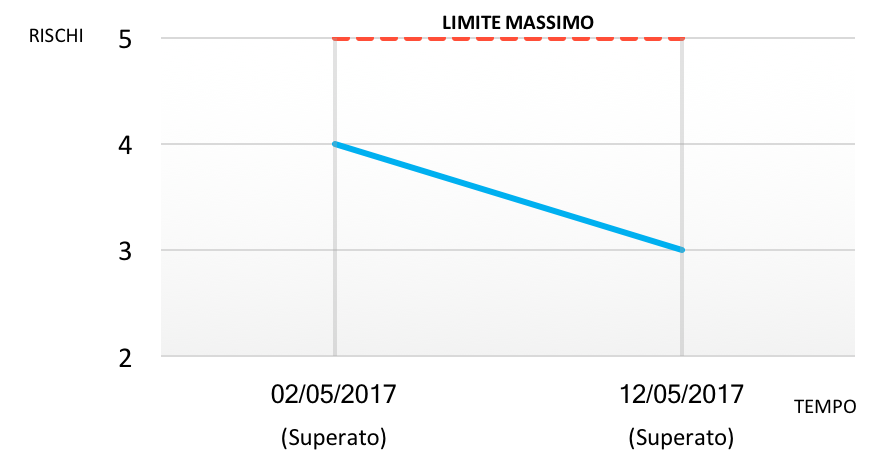
\includegraphics{grafici/Rischi.png}
			\caption{Riscontro dei rischi nei due periodi - RA}
			\label{fig:rischi}
		\end{figure}\mbox{}\\

		\begin{longtable}[c] { >{\centering\arraybackslash}p{3cm} >{\centering\arraybackslash}p{3cm} }
			\toprule
					\textbf{Valore} & \textbf{Esito} \\
				\midrule
					3 & superato \\
				\bottomrule
			\caption{Rischi non preventivati - RA}
		\end{longtable}\mbox{}\\

		\textbf{Copertura requisiti obbligatori}
		\begin{figure}[!h]
			\centering
			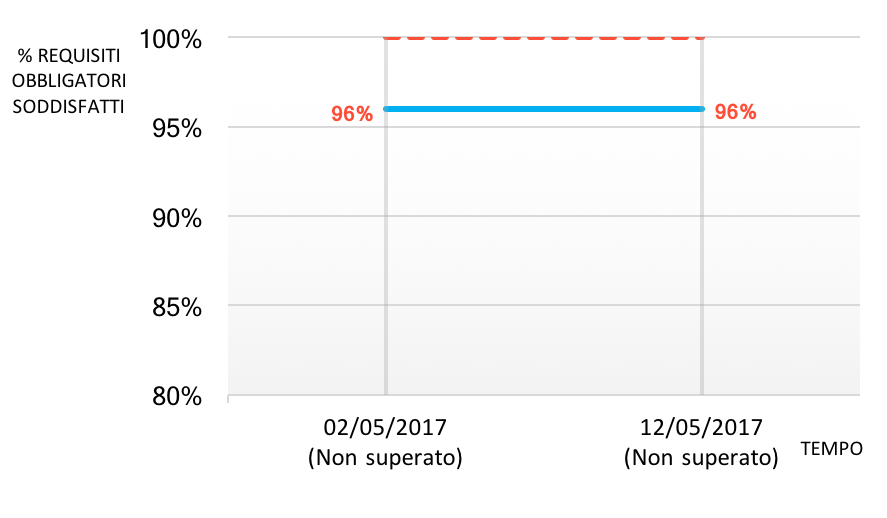
\includegraphics{grafici/Requisiti.png}
			\caption{Soddisfacimento requisiti obbligatori nei due periodi - RA}
			\label{fig:requisiti}
		\end{figure}\mbox{}\\

		\begin{longtable}[c] { >{\centering\arraybackslash}p{3cm} >{\centering\arraybackslash}p{3cm} }
			\toprule
					\textbf{Valore} & \textbf{Esito} \\
				\midrule
					96\% & Non superato \\
				\bottomrule
			\caption{Copertura requisiti obbligatori - RA}
		\end{longtable}\mbox{}\\

		\newpage
		\textbf{Structural Fan-In}
		\begin{figure}[!h]
			\centering
			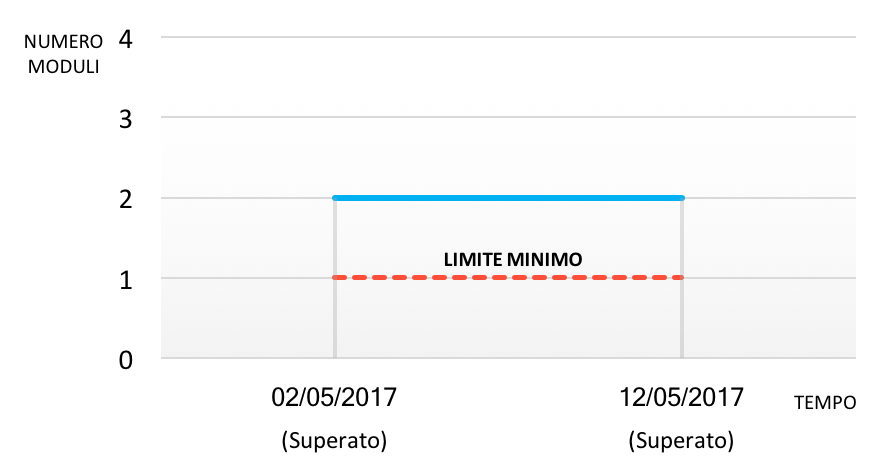
\includegraphics{grafici/Fan-in.png}
			\caption{Valore di Fan-in nei due periodi - RA}
			\label{fig:fanIn}
		\end{figure}\mbox{}\\

		\begin{longtable}[c] { >{\centering\arraybackslash}p{3cm} >{\centering\arraybackslash}p{3cm} }
			\toprule
					\textbf{Valore} & \textbf{Esito} \\
				\midrule
					2 & superato \\
				\bottomrule
			\caption{Structural Fan-In - RA}
		\end{longtable}\mbox{}\\

		\newpage
		\textbf{Structural Fan-Out}
		\begin{figure}[!h]
			\centering
			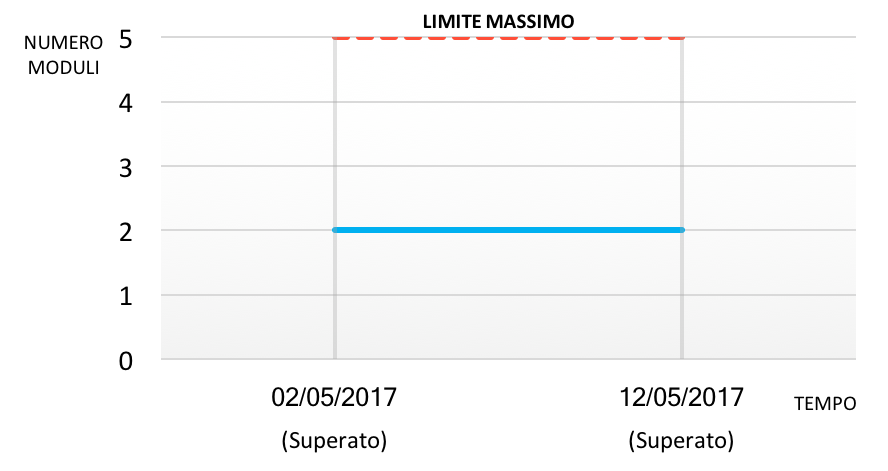
\includegraphics{grafici/Fan-out.png}
			\caption{Valore di Fan-out nei due periodi - RA}
			\label{fig:fanOut}
		\end{figure}\mbox{}\\
		
		\begin{longtable}[c] { >{\centering\arraybackslash}p{3cm} >{\centering\arraybackslash}p{3cm} }
			\toprule
					\textbf{Valore} & \textbf{Esito} \\
				\midrule
					2 & Superato \\
				\bottomrule
			\caption{Structural Fan-Out - RA}
		\end{longtable}\mbox{}\\

		\newpage
		\textbf{Numero di metodi per classe}\acapo
		Controllate tutte le classi, il numero massimo di metodi calcolato nei due periodi di questa revisione è il seguente:
		\begin{figure}[!h]
			\centering
			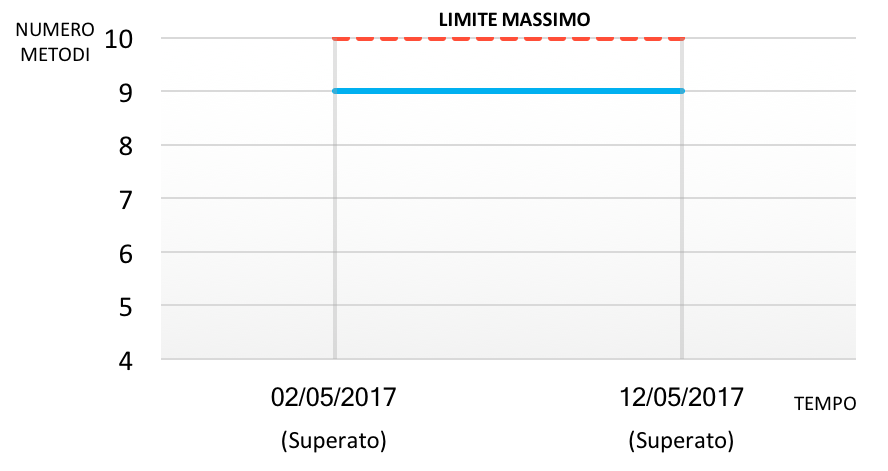
\includegraphics{grafici/Metodi.png}
			\caption{Numero di metodi massimo nei due periodi - RA}
			\label{fig:metodi}
		\end{figure}\mbox{}\\

		\begin{longtable}[c] { >{\centering\arraybackslash}p{3cm} >{\centering\arraybackslash}p{3cm} }
			\toprule
					\textbf{Valore} & \textbf{Esito} \\
				\midrule
					9 & Superato \\
				\bottomrule
			\caption{Numero di metodi per classe - RA}
		\end{longtable}\mbox{}\\


		\newpage
		\textbf{Numero di parametri per metodo}
		\begin{figure}[!h]
			\centering
			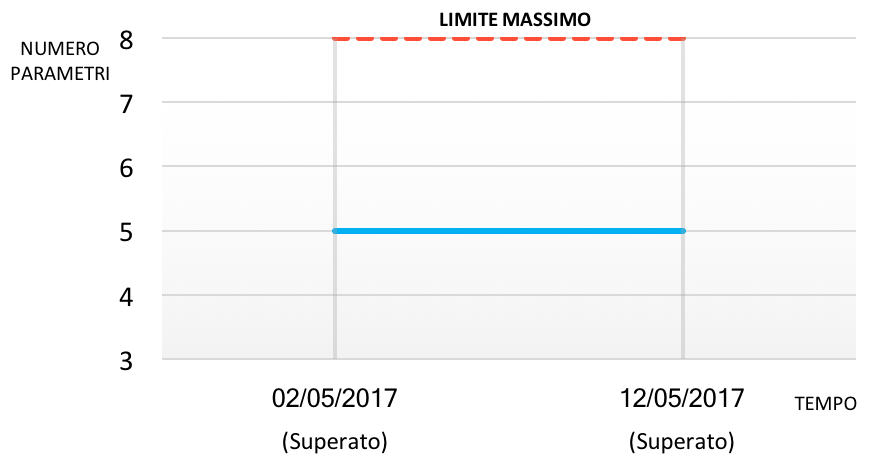
\includegraphics{grafici/Parametri.png}
			\caption{Numero di parametri massimo nei due periodi - RA}
			\label{fig:parametri}
		\end{figure}\mbox{}\\

		\begin{longtable}[c] { >{\centering\arraybackslash}p{3cm} >{\centering\arraybackslash}p{3cm} }
			\toprule
					\textbf{Valore} & \textbf{Esito} \\
				\midrule
					5 & Superato \\
				\bottomrule
			\caption{Numero di parametri per metodo - RA}
		\end{longtable}\mbox{}\\

		\newpage
		\textbf{Complessità ciclomatica}
		\begin{figure}[!h]
			\centering
			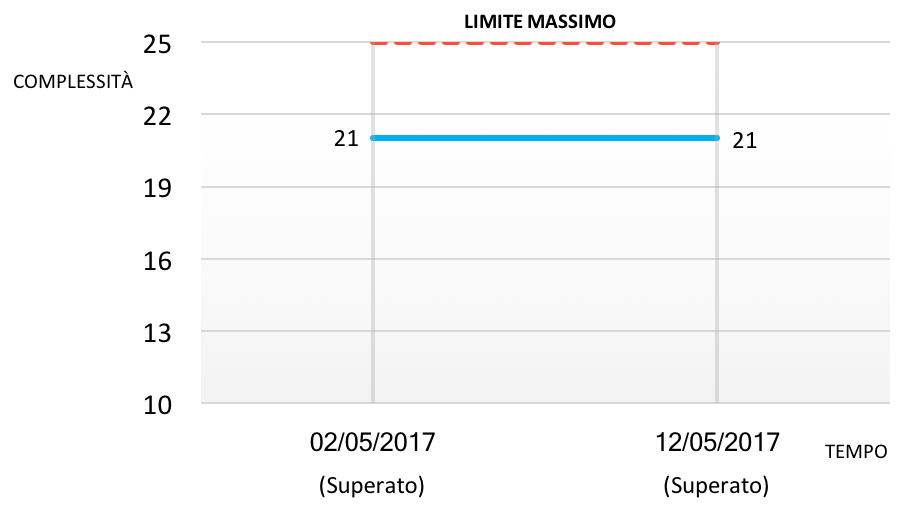
\includegraphics{grafici/Ciclomatica.png}
			\caption{Complessità ciclomatica nei due periodi - RA}
			\label{fig:ciclomatica}
		\end{figure}\mbox{}\\
		
		\begin{longtable}[c] { >{\centering\arraybackslash}p{3cm} >{\centering\arraybackslash}p{3cm} }
			\toprule
					\textbf{Valore} & \textbf{Esito} \\
				\midrule
					21 & Superato \\
				\bottomrule
			\caption{Complessità ciclomatica - RA}
		\end{longtable}\mbox{}\\

		\newpage
		\textbf{Halstead difficulty per function}
		\begin{figure}[!h]
			\centering
			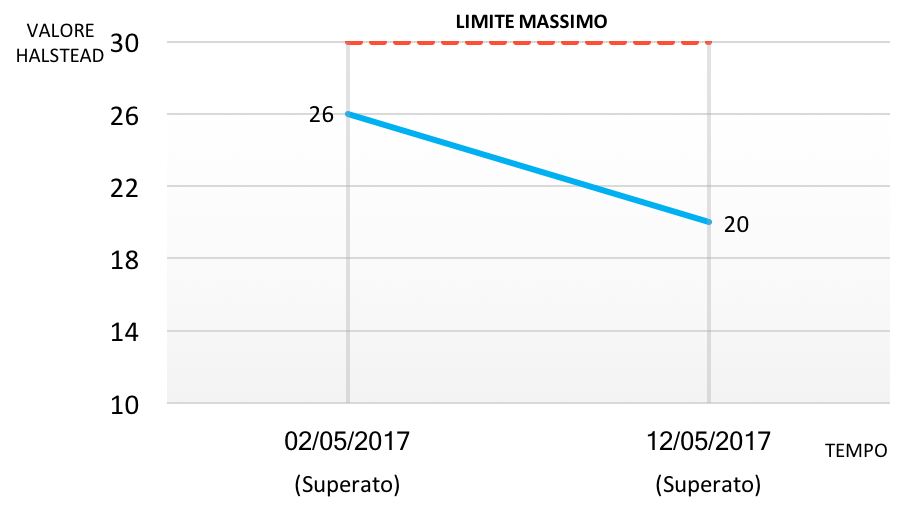
\includegraphics{grafici/HalsteadDiff.png}
			\caption{Halstead difficulty nei due periodi - RA}
			\label{fig:halsteadDiff}
		\end{figure}\mbox{}\\
		
		\begin{longtable}[c] { >{\centering\arraybackslash}p{3cm} >{\centering\arraybackslash}p{3cm} }
			\toprule
					\textbf{Valore} & \textbf{Esito} \\
				\midrule
					20 & Superato \\
				\bottomrule
			\caption{Halstead difficulty per function - RA}
		\end{longtable}\mbox{}\\

		\newpage
		\textbf{Halstead volume per function}
		\begin{figure}[!h]
			\centering
			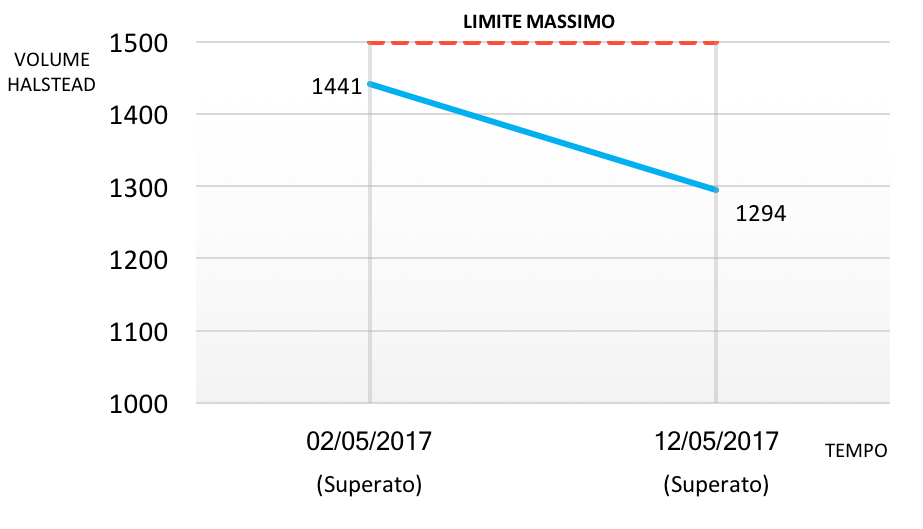
\includegraphics{grafici/HalsteadVol.png}
			\caption{Halstead volume nei due periodi - RA}
			\label{fig:halsteadVol}
		\end{figure}\mbox{}\\
		
		\begin{longtable}[c] { >{\centering\arraybackslash}p{3cm} >{\centering\arraybackslash}p{3cm} }
			\toprule
					\textbf{Valore} & \textbf{Esito} \\
				\midrule
					1294 & Superato \\
				\bottomrule
			\caption{Halstead volume per function - RA}
		\end{longtable}\mbox{}\\


		\newpage
		\textbf{Halstead effort per function}
		\begin{figure}[!h]
			\centering
			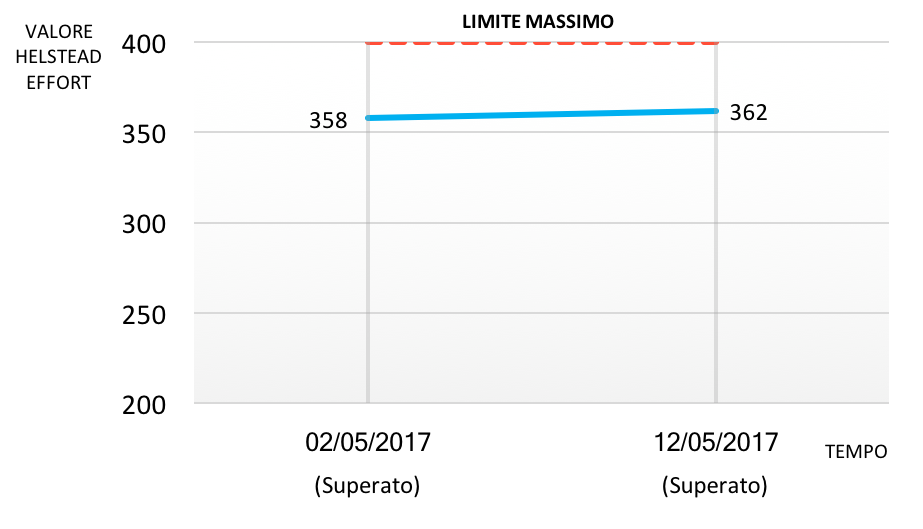
\includegraphics{grafici/HalsteadEffort.png}
			\caption{Halstead effort nei due periodi - RA}
			\label{fig:halsteadeffort}
		\end{figure}\mbox{}\\

		\begin{longtable}[c] { >{\centering\arraybackslash}p{3cm} >{\centering\arraybackslash}p{3cm} }
			\toprule
					\textbf{Valore} & \textbf{Esito} \\
				\midrule
					362 & Superato \\
				\bottomrule
			\caption{Halstead effort per function - RA}
		\end{longtable}\mbox{}\\

		\newpage
		\textbf{Maintainability index}
		\begin{figure}[!h]
			\centering
			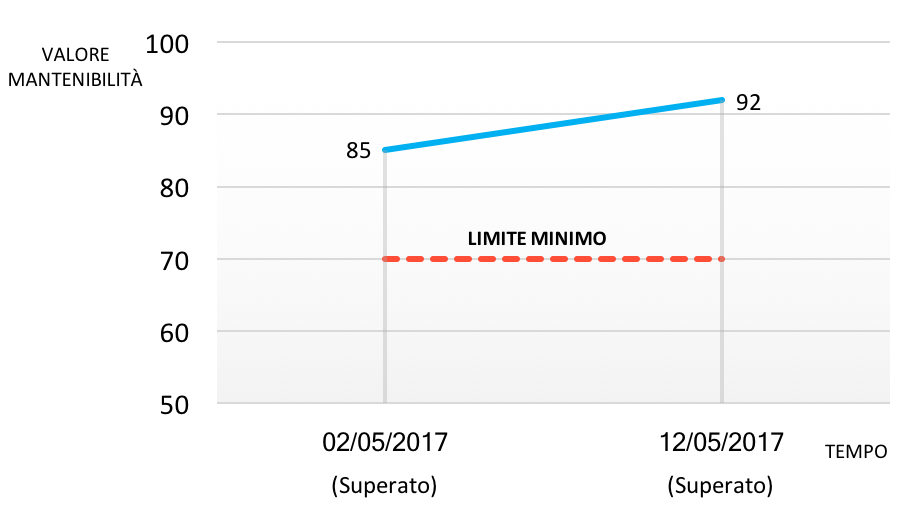
\includegraphics{grafici/Mantenibilita.png}
			\caption{Indice di mantenibilità nei due periodi - RA}
			\label{fig:maintain}
		\end{figure}\mbox{}\\

		\begin{longtable}[c] { >{\centering\arraybackslash}p{3cm} >{\centering\arraybackslash}p{3cm} }
			\toprule
					\textbf{Valore} & \textbf{Esito} \\
				\midrule
					92 & Superato \\
				\bottomrule
			\caption{Maintainability index - RA}
		\end{longtable}\mbox{}\\


		\newpage
		\textbf{Produttività di codifica}
		\begin{figure}[!h]
			\centering
			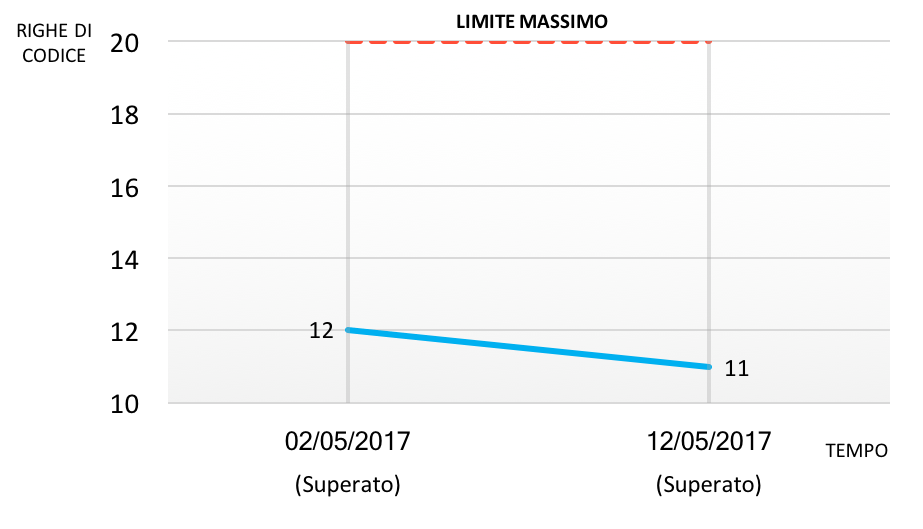
\includegraphics{grafici/Codifica.png}
			\caption{Produttività di codifica nei due periodi - RA}
			\label{fig:codifica}
		\end{figure}\mbox{}\\

		\begin{longtable}[c] { >{\centering\arraybackslash}p{3cm} >{\centering\arraybackslash}p{3cm} }
			\toprule
					\textbf{Valore} & \textbf{Esito} \\
				\midrule
					11 & Superato \\
				\bottomrule
			\caption{Produttività di codifica - RA}
		\end{longtable}\mbox{}\\

		\newpage
		\textbf{Numero di livelli di annidamento}
		\begin{figure}[!h]
			\centering
			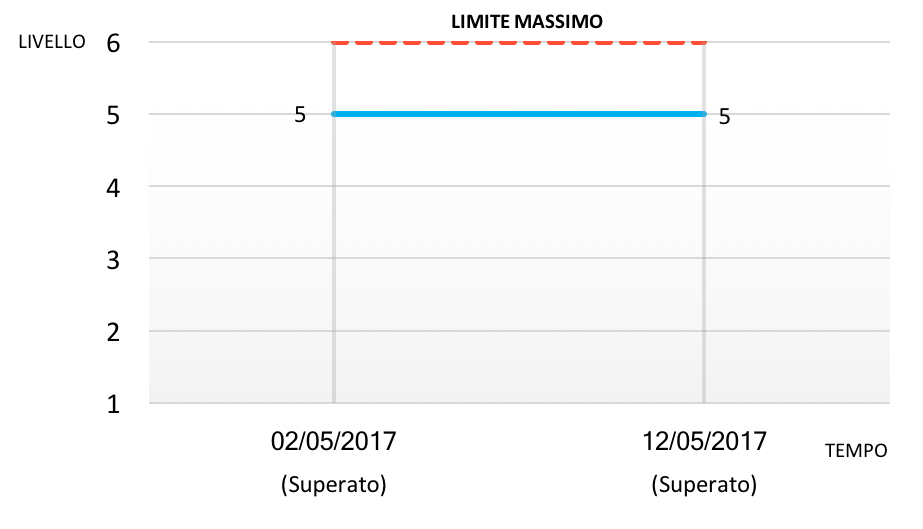
\includegraphics{grafici/Annidamento.png}
			\caption{Livello di annidamento massimo nei due periodi - RA}
			\label{fig:annidamento}
		\end{figure}\mbox{}\\

		\begin{longtable}[c] { >{\centering\arraybackslash}p{3cm} >{\centering\arraybackslash}p{3cm} }
			\toprule
					\textbf{Valore} & \textbf{Esito} \\
				\midrule
					5 & Superato \\
				\bottomrule
			\caption{Numero di livelli di annidamento - RA}
		\end{longtable}\mbox{}\\

		\newpage
		\textbf{Variabili inutilizzate}
		\begin{longtable}[c] { >{\centering\arraybackslash}p{3cm} >{\centering\arraybackslash}p{3cm} >{\centering\arraybackslash}p{3cm} }
			\toprule
					\textbf{Valore} & \textbf{Data} & \textbf{Esito} \\
				\midrule
					0 & 02/05/2017 & Superato \\
				\midrule
					0 & 12/05/2017 & Superato \\
				\bottomrule
			\caption{Variabili inutilizzate: riscontro nei due periodi - RA}
		\end{longtable}\mbox{}\\

		\begin{longtable}[c] { >{\centering\arraybackslash}p{3cm} >{\centering\arraybackslash}p{3cm} }
			\toprule
					\textbf{Valore} & \textbf{Esito} \\
				\midrule
					0 & Superato \\
				\bottomrule
			\caption{Variabili inutilizzate - RA}
		\end{longtable}\mbox{}\\

		\textbf{Componenti integrate}
		\begin{figure}[!h]
			\centering
			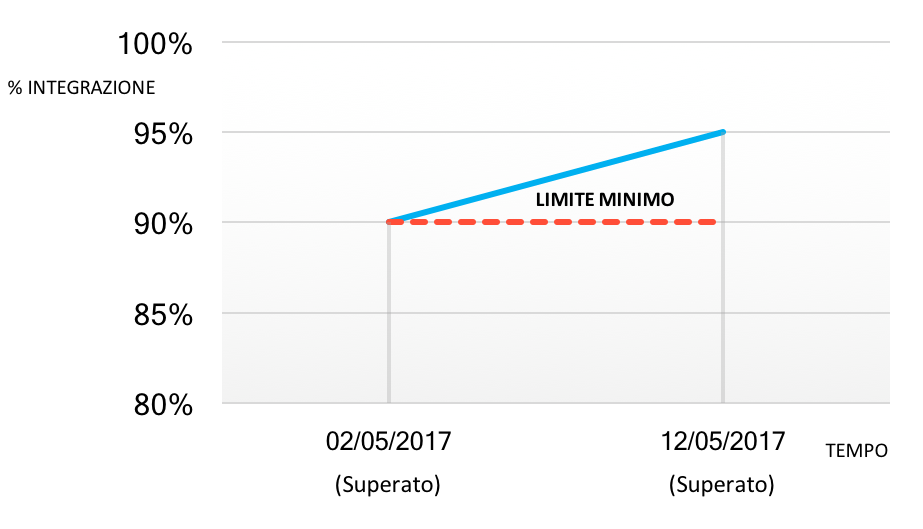
\includegraphics{grafici/Integrazione.png}
			\caption{Integrazione delle componenti nei due periodi - RA}
			\label{fig:integration}
		\end{figure}\mbox{}\\

		\begin{longtable}[c] { >{\centering\arraybackslash}p{3cm} >{\centering\arraybackslash}p{3cm} }
			\toprule
					\textbf{Valore} & \textbf{Esito} \\
				\midrule
					95\% & Superato \\
				\bottomrule
			\caption{Componenti integrate - RA}
		\end{longtable}\mbox{}\\

		\textbf{Test di unità eseguiti}
		\begin{figure}[!h]
			\centering
			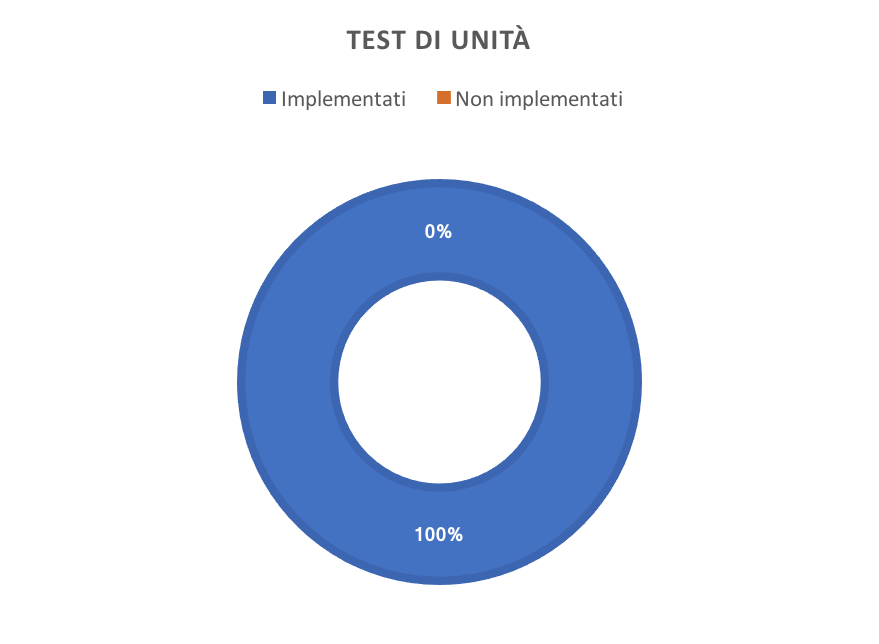
\includegraphics{grafici/TU.png}
			\caption{\% di test di unità eseguiti nei due periodi - RA}
			\label{fig:integration}
		\end{figure}\mbox{}\\

		\begin{longtable}[c] { >{\centering\arraybackslash}p{3cm} >{\centering\arraybackslash}p{3cm} }
			\toprule
					\textbf{Valore} & \textbf{Esito} \\
				\midrule
					100\% & Superato \\
				\bottomrule
			\caption{Test di unità eseguiti - RA}
		\end{longtable}\mbox{}\\

		\newpage
		\textbf{Test di integrazione eseguiti}
		\begin{figure}[!h]
			\centering
			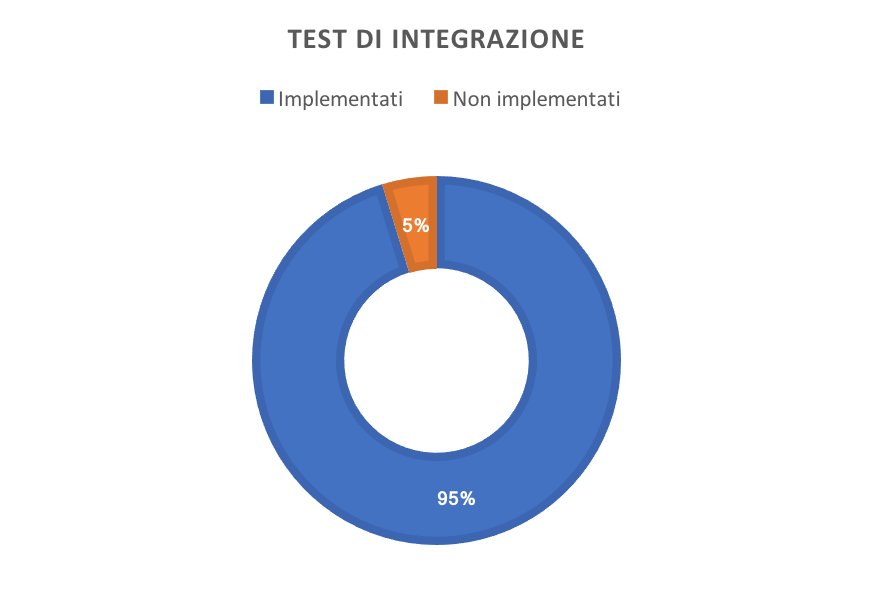
\includegraphics{grafici/TI.png}
			\caption{\% di test di integrazione eseguiti nei due periodi - RA}
			\label{fig:integration}
		\end{figure}\mbox{}\\

		\begin{longtable}[c] { >{\centering\arraybackslash}p{3cm} >{\centering\arraybackslash}p{3cm} }
			\toprule
					\textbf{Valore} & \textbf{Esito} \\
				\midrule
					100\% & Superato \\
				\bottomrule
			\caption{Test di integrazione eseguiti - RA}
		\end{longtable}\mbox{}\\

		\newpage
		\textbf{Test di sistema eseguiti}
		\begin{figure}[!h]
			\centering
			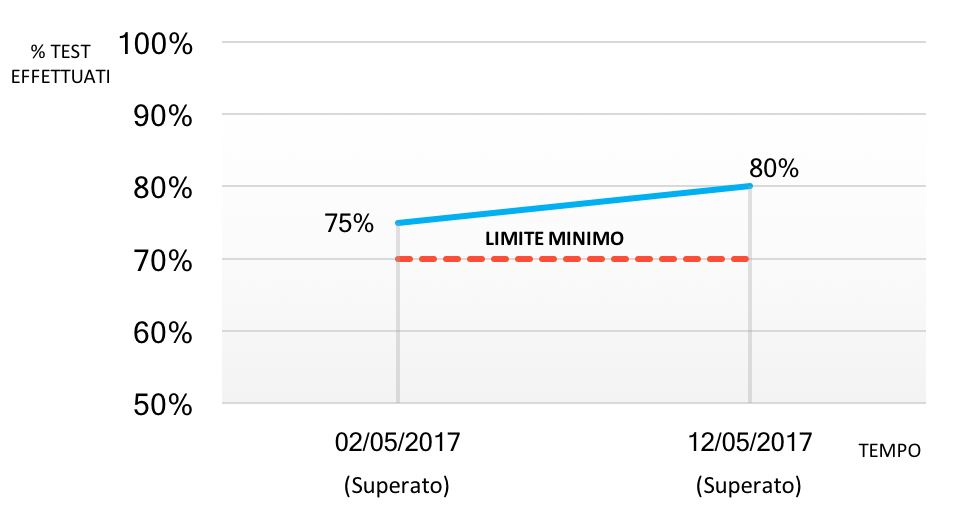
\includegraphics{grafici/TS.png}
			\caption{\% di test di sistema effettuati nei due periodi - RA}
			\label{fig:integration}
		\end{figure}\mbox{}\\
		
		\begin{longtable}[c] { >{\centering\arraybackslash}p{3cm} >{\centering\arraybackslash}p{3cm} }
			\toprule
					\textbf{Valore} & \textbf{Esito} \\
				\midrule
					80\% & Superato \\
				\bottomrule
			\caption{Test di sistema eseguiti - RA}
		\end{longtable}\mbox{}\\

		\newpage
		\textbf{Copertura dei test}
		\begin{figure}[!h]
			\centering
			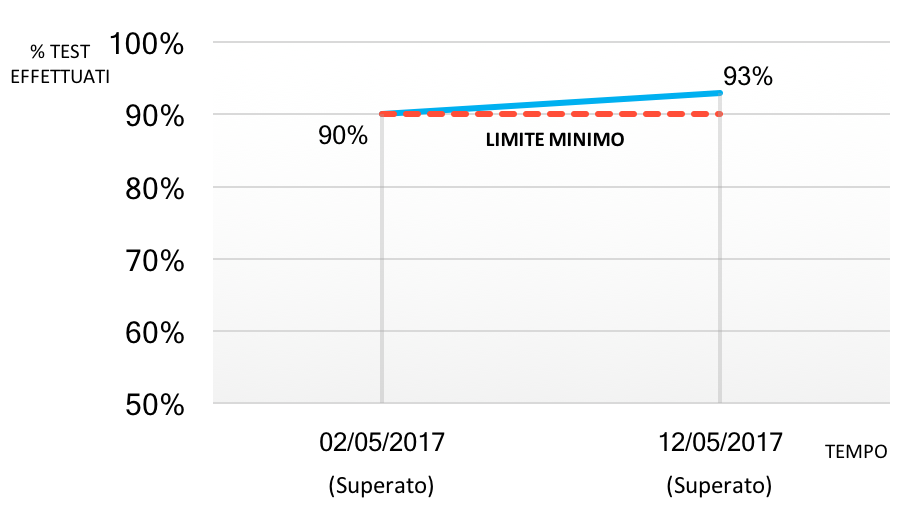
\includegraphics{grafici/CoperturaTest.png}
			\caption{\% di test di copertura totale dei test effettuati nei due periodi - RA}
			\label{fig:integration}
		\end{figure}\mbox{}\\
		
		\begin{longtable}[c] { >{\centering\arraybackslash}p{3cm} >{\centering\arraybackslash}p{3cm} }
			\toprule
					\textbf{Valore} & \textbf{Esito} \\
				\midrule
					93\% & Superato \\
				\bottomrule
			\caption{Copertura dei test - RA}
		\end{longtable}\mbox{}\\

		\newpage
		\textbf{Indice Gulpease}
		\begin{figure}[!h]
			\centering
			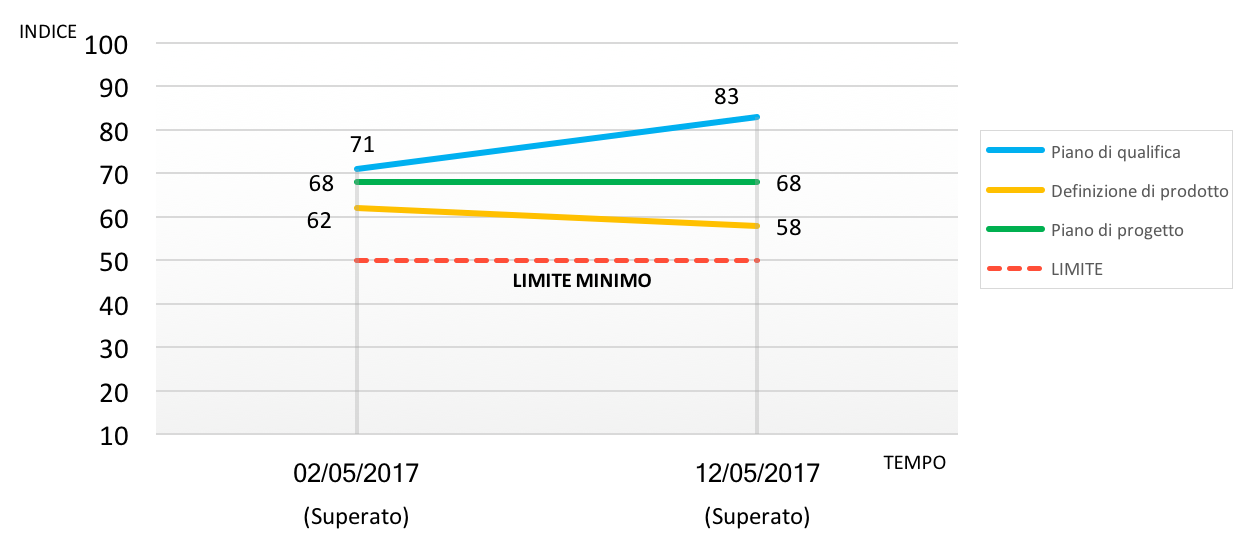
\includegraphics[width=\textwidth]{grafici/Gulpease1.png}
			\caption{Indice di gulpease per alcuni documenti nei due periodi - RA}
			\label{fig:gulpease1}
		\end{figure}\mbox{}\\

		\textbf{Indice Gulpease}
		\begin{longtable}[c] { p{5cm} >{\centering\arraybackslash}p{3cm} >{\centering\arraybackslash}p{3cm}}
			\toprule
					\textbf{Documento} & \textbf{Gulpease} & \textbf{Esito} \\
				\midrule
					\pianodiqualificaRA & 83 & Superato \\
					\definizionediprodottoRA & 58 & Superato \\
					\pianodiprogettoRA & 58 & Superato \\
				\bottomrule
			\caption{Indice Gulpease 1a parte - RA}
		\end{longtable}\mbox{}\\

\newpage

		\begin{figure}[!h]
			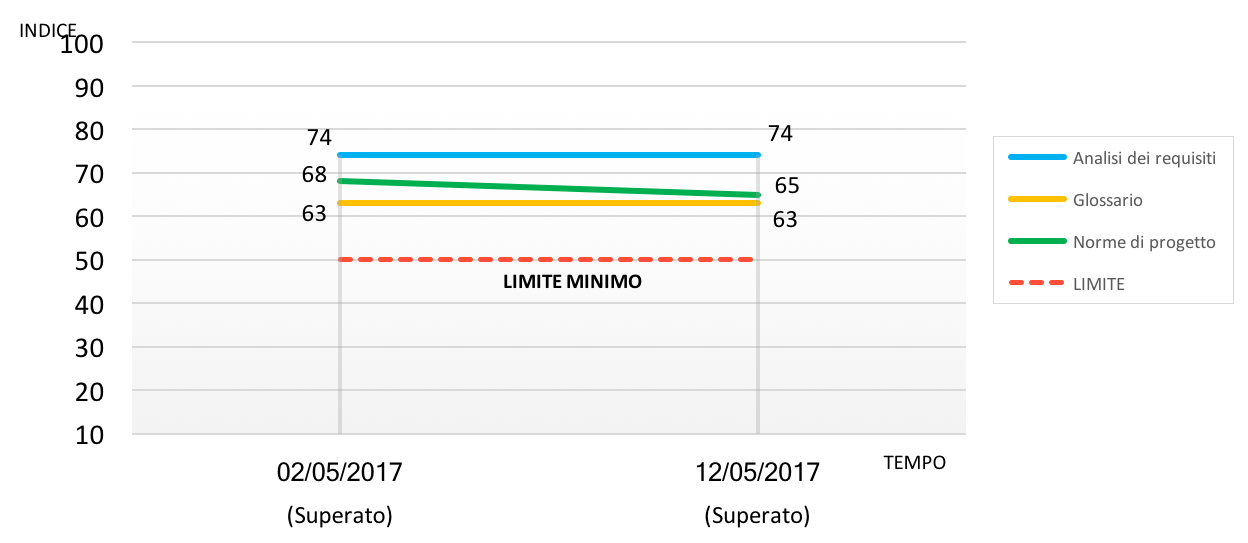
\includegraphics[width=\textwidth]{grafici/Gulpease2.png}
			\caption{Indice di gulpease per alcuni documenti due periodi - RA}
			\label{fig:gulpease2}
		\end{figure}\mbox{}\\

		\textbf{Indice Gulpease}
		\begin{longtable}[c] { p{5cm} >{\centering\arraybackslash}p{3cm} >{\centering\arraybackslash}p{3cm}}
			\toprule
					\textbf{Documento} & \textbf{Gulpease} & \textbf{Esito} \\
				\midrule
					\analisideirequisitiRA & 74 & Superato \\
					\glossarioRA & 63 & Superato \\
					\normediprogettoRA & 58 & Superato \\
				\bottomrule
			\caption{Indice Gulpease 2a parte - RA}
		\end{longtable}\mbox{}\\

		
	\newpage

		\textbf{Errori ortografici rilevati e non corretti}
		\begin{longtable}[c] { >{\centering\arraybackslash}p{3cm} >{\centering\arraybackslash}p{3cm} >{\centering\arraybackslash}p{3cm} }
			\toprule
					\textbf{Valore} & \textbf{Data} & \textbf{Esito} \\
				\midrule
					0\% & 02/05/2017 & Superato \\
				\midrule
					0\% & 12/05/2017 & Superato \\
				\bottomrule
			\caption{Errori ortografici rilevati e non corretti - RA}
		\end{longtable}\mbox{}\\

		\textbf{Errori concettuali rilevati e non corretti}
		\begin{longtable}[c] { >{\centering\arraybackslash}p{3cm} >{\centering\arraybackslash}p{3cm} >{\centering\arraybackslash}p{3cm} }
			\toprule
					\textbf{Valore} & \textbf{Data} & \textbf{Esito} \\
				\midrule
					0\% & 02/05/2017 & Superato \\
				\midrule
					0\% & 12/05/2017 & Superato \\
				\bottomrule
			\caption{Errori concettuali rilevati e non corretti - RA}
		\end{longtable}\mbox{}\\

		\textbf{Statement coverage}
		\begin{figure}[!h]
			\centering
			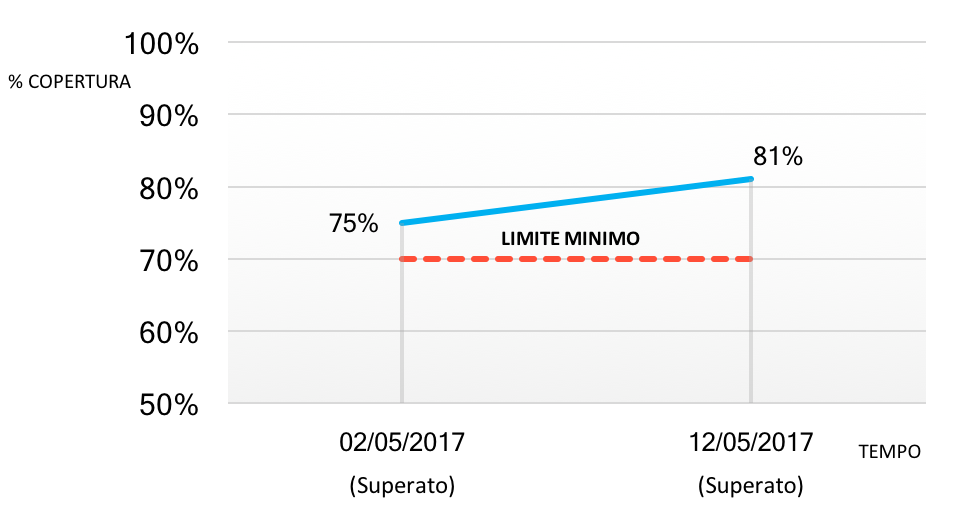
\includegraphics{grafici/Statement.png}
			\caption{Statement coverage nei due periodi - RA}
			\label{fig:integration}
		\end{figure}\mbox{}\\

		\begin{longtable}[c] { >{\centering\arraybackslash}p{3cm} >{\centering\arraybackslash}p{3cm} }
			\toprule
					\textbf{Valore} & \textbf{Esito} \\
				\midrule
					81\% & Superato \\
				\bottomrule
			\caption{Statement coverage - RA}
		\end{longtable}\mbox{}\\


		\textbf{Branch coverage}
		\begin{figure}[!h]
			\centering
			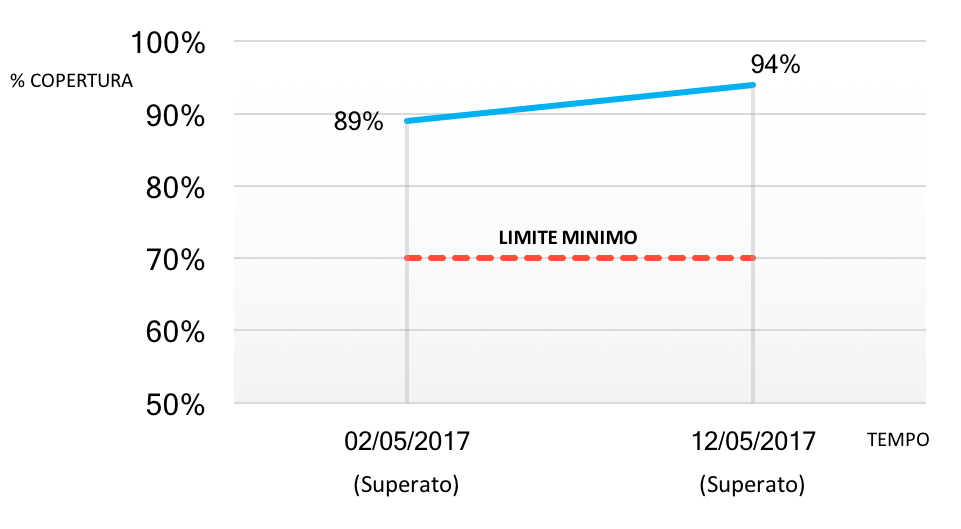
\includegraphics{grafici/Branch.png}
			\caption{Branch coverage nei due periodi - RA}
			\label{fig:integration}
		\end{figure}\mbox{}\\

		\begin{longtable}[c] { >{\centering\arraybackslash}p{3cm} >{\centering\arraybackslash}p{3cm} }
			\toprule
					\textbf{Valore} & \textbf{Esito} \\
				\midrule
					94\% & Superato \\
				\bottomrule
			\caption{Branch coverage - RA}
		\end{longtable}\mbox{}\\

\newpage

	\paragraph{Riscontri di qualità di prodotto}\acapo\acapo
	Di seguito sono presentati graficamente, tramite \textit{line charts}, i risultati qualitativi sul prodotto finale sviluppato.
	Questi riscontri sono misurati in base a valori obiettivo precedentemente fissati in fase di progettazione e descritti nella sottosezione apposita (\ref{ssec:qualitaprodotto}) all'inizio di questo documento.
	\vspace*{0,7cm}

	\textbf{Completezza dell’implementazione funzionale}
	\begin{figure}[!h]
		\centering
		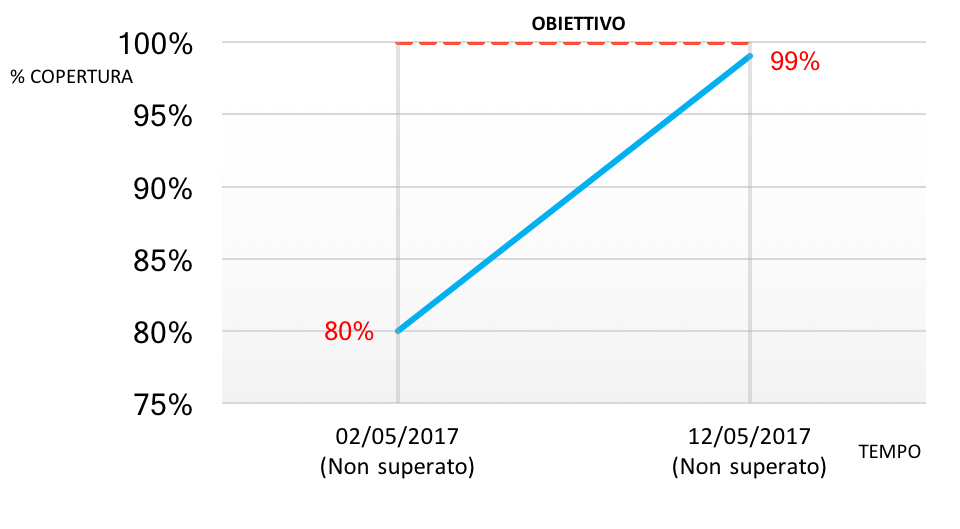
\includegraphics{grafici/Completezza.png}
		\caption{Completezza funzionale del prodotto nei due periodi - RA}
		\label{fig:completezza}
	\end{figure}\mbox{}\\

	\begin{longtable}[c] { >{\centering\arraybackslash}p{3cm} >{\centering\arraybackslash}p{3cm} }
		\toprule
				\textbf{Valore} & \textbf{Esito} \\
			\midrule
				99\% & Non superato \\
			\bottomrule
		\caption{Completezza dell’implementazione funzionale - RA}
	\end{longtable}\mbox{}\\

	\newpage
	\textbf{Accuratezza rispetto alle attese}
	\begin{figure}[!h]
		\centering
		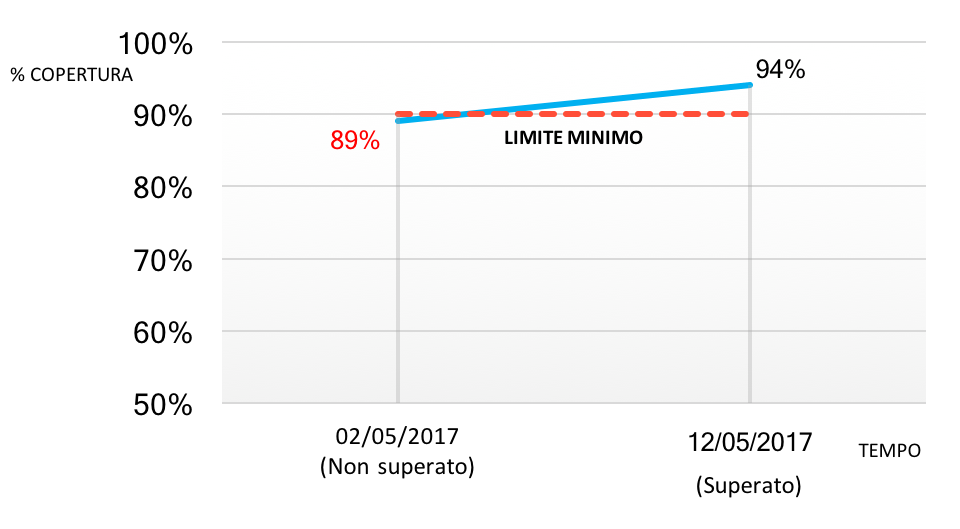
\includegraphics{grafici/Attese.png}
		\caption{Accuratezza alle attese nei due periodi - RA}
		\label{fig:attese}
	\end{figure}\mbox{}\\

	\begin{longtable}[c] { >{\centering\arraybackslash}p{3cm} >{\centering\arraybackslash}p{3cm} }
		\toprule
				\textbf{Valore} & \textbf{Esito} \\
			\midrule
				94\% & Superato \\
			\bottomrule
		\caption{Accuratezza rispetto alle attese - RA}
	\end{longtable}\mbox{}\\

	\textbf{Controllo degli accessi}\acapo\acapo
	Il limite di accessi illegali imposto in pianificazione è del 10\%.
	\begin{longtable}[c] { >{\centering\arraybackslash}p{3cm} >{\centering\arraybackslash}p{3cm} >{\centering\arraybackslash}p{3cm} }
		\toprule
			\textbf{Valore} & \textbf{Data} & \textbf{Esito} \\
			\midrule
				0\% & 02/05/2017 & Superato \\
			\midrule
				0\% & 12/05/2017 & Superato \\
			\bottomrule
		\caption{Controllo degli accessi - RA}
	\end{longtable}\mbox{}\\	
		
	
	\textbf{Copertura requisiti desiderabili}
	\begin{figure}[!h]
		\centering
		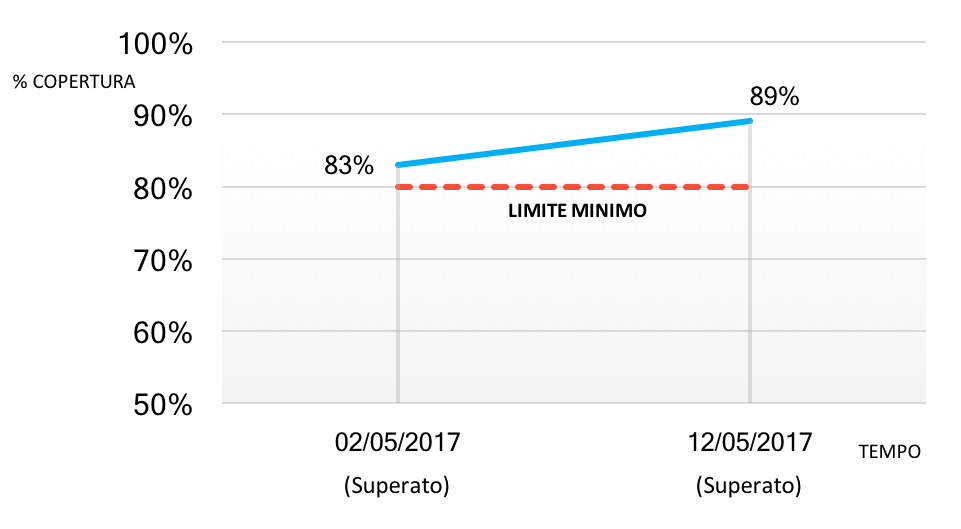
\includegraphics{grafici/Desiderabili.png}
		\caption{Copertura dei requisiti desiderabili del prodotto nei due periodi - RA}
		\label{fig:desiderabili}
	\end{figure}\mbox{}\\

	\begin{longtable}[c] { >{\centering\arraybackslash}p{3cm} >{\centering\arraybackslash}p{3cm} }
		\toprule
				\textbf{Valore} & \textbf{Esito} \\
			\midrule
				89\% & Superato \\
			\bottomrule
		\caption{Copertura requisiti desiderabili - RA}
	\end{longtable}\mbox{}\\

	\textbf{Densità di failure}\acapo\acapo
	Il limite massimo per la densità di failure durante i test è imposto al 10\%
	\begin{longtable}[c] { >{\centering\arraybackslash}p{3cm} >{\centering\arraybackslash}p{3cm} >{\centering\arraybackslash}p{3cm} }
		\toprule
			\textbf{Valore} & \textbf{Data} & \textbf{Esito} \\
			\midrule
				2\% & 02/05/2017 & Superato \\
			\midrule
				2\% & 12/05/2017 & Superato \\
			\bottomrule
		\caption{Densità di failure - RA}
	\end{longtable}\mbox{}\\

\newpage
	\textbf{Blocco operazioni non corrette}
	\begin{figure}[!h]
		\centering
		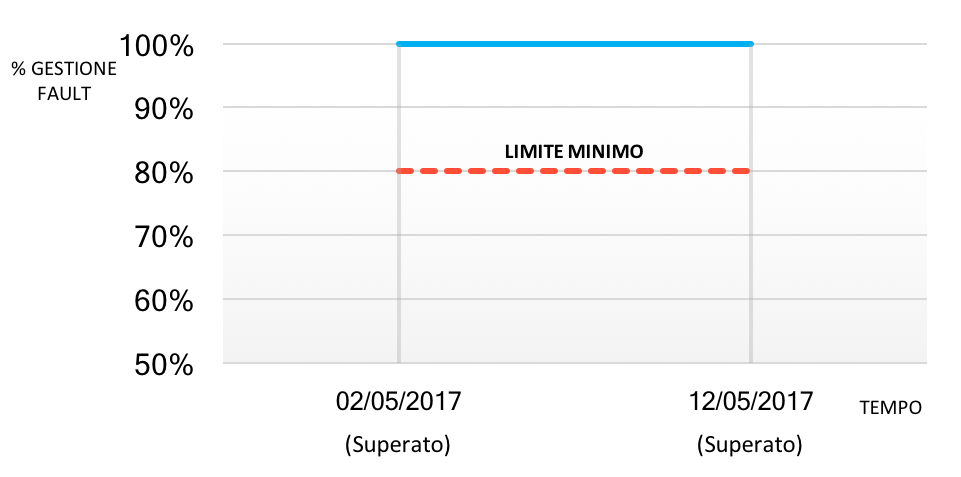
\includegraphics{grafici/Blocco.png}
		\caption{\% di operazioni non corrette nei due periodi - RA}
		\label{fig:blocco}
	\end{figure}\mbox{}\\

	\begin{longtable}[c] { >{\centering\arraybackslash}p{3cm} >{\centering\arraybackslash}p{3cm} }
		\toprule
				\textbf{Valore} & \textbf{Esito} \\
			\midrule
				100\% & Superato \\
			\bottomrule
		\caption{Blocco operazioni non corrette - RA}
	\end{longtable}\mbox{}\\

	\newpage
	\textbf{Comprensibilità delle funzioni offerte}
	\begin{figure}[!h]
		\centering
		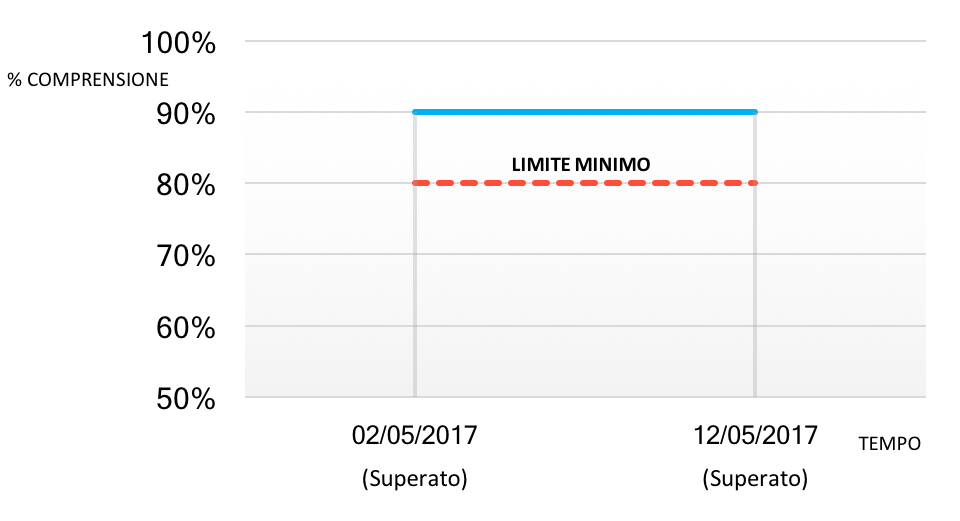
\includegraphics{grafici/Comprensione.png}
		\caption{Comprensione delle funzionalità del prodotto nei due periodi - RA}
		\label{fig:comprensione}
	\end{figure}\mbox{}\\	

	\begin{longtable}[c] { >{\centering\arraybackslash}p{3cm} >{\centering\arraybackslash}p{3cm} }
		\toprule
				\textbf{Valore} & \textbf{Esito} \\
			\midrule
				90\% & Superato \\
			\bottomrule
		\caption{Comprensibilità delle funzioni offerte - RA}
	\end{longtable}\mbox{}\\

	\newpage
	\textbf{Facilità di apprendimento}
	\begin{figure}[!h]
		\centering
		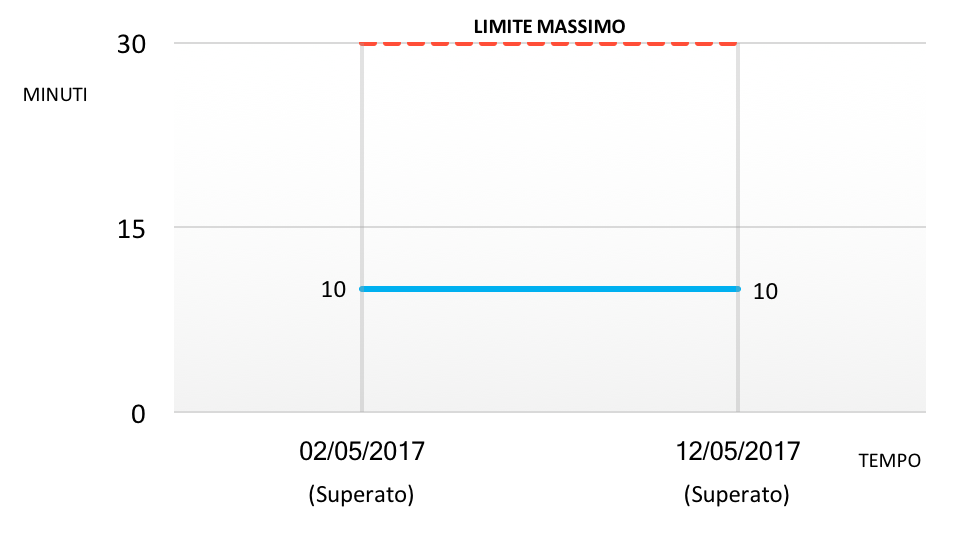
\includegraphics{grafici/Facilita.png}
		\caption{Facilità di apprendimento nei due periodi - RA}
		\label{fig:apprendimento}
	\end{figure}\mbox{}\\

	\begin{longtable}[c] { >{\centering\arraybackslash}p{3cm} >{\centering\arraybackslash}p{3cm} }
		\toprule
				\textbf{Valore} & \textbf{Esito} \\
			\midrule
				10 & Superato \\
			\bottomrule
		\caption{Facilità di apprendimento - RA}
	\end{longtable}\mbox{}\\

	\newpage
	\textbf{Consistenza operazionale in uso}
	\begin{figure}[!h]
		\centering
		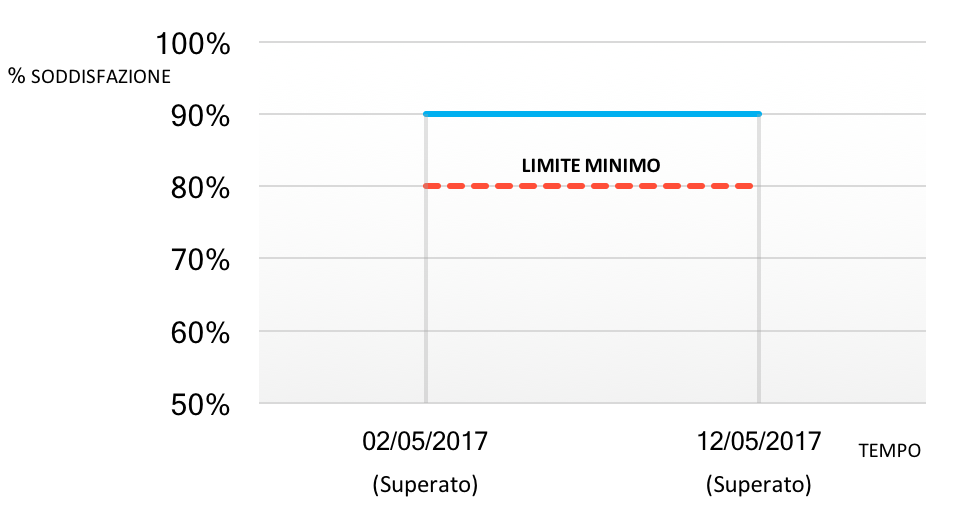
\includegraphics{grafici/Consistenza.png}
		\caption{Consistenza delle operazioni del prodotto nei due periodi - RA}
		\label{fig:consistenza}
	\end{figure}\mbox{}\\

	\begin{longtable}[c] { >{\centering\arraybackslash}p{3cm} >{\centering\arraybackslash}p{3cm} }
		\toprule
				\textbf{Valore} & \textbf{Esito} \\
			\midrule
				90\% & Superato \\
			\bottomrule
		\caption{Consistenza delle operazioni del prodotto nei due periodi - RA}
	\end{longtable}\mbox{}\\

	\newpage
	\textbf{Capacità di analisi di failure}
	\begin{figure}[!h]
		\centering
		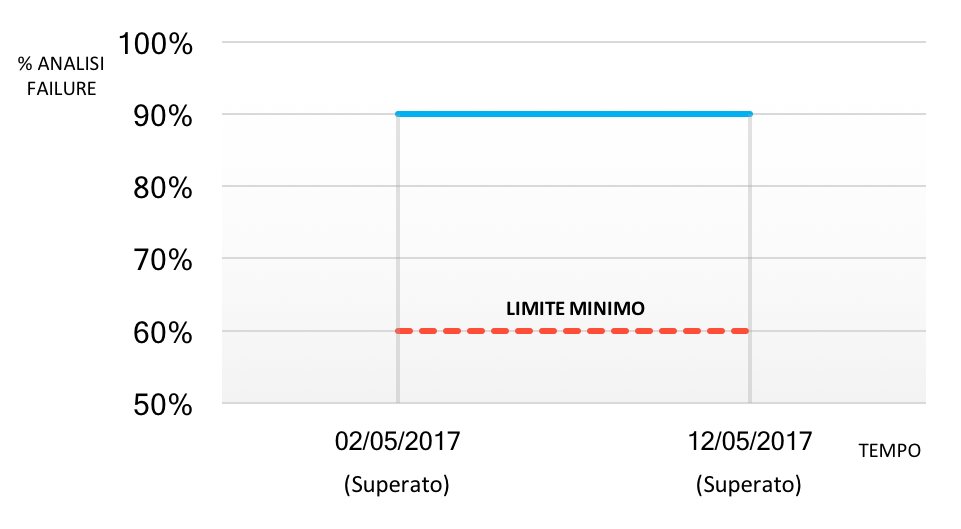
\includegraphics{grafici/Failure.png}
		\caption{Capacità di analisi di failure - RA}
		\label{fig:failure}
	\end{figure}\mbox{}\\

	\begin{longtable}[c] { >{\centering\arraybackslash}p{3cm} >{\centering\arraybackslash}p{3cm} }
		\toprule
				\textbf{Valore} & \textbf{Esito} \\
			\midrule
				90\% & Superato \\
			\bottomrule
		\caption{Capacità di analisi di failure - RA}
	\end{longtable}\mbox{}\\

	\newpage
	\textbf{Impatto delle modifiche}
	\begin{figure}[!h]
		\centering
		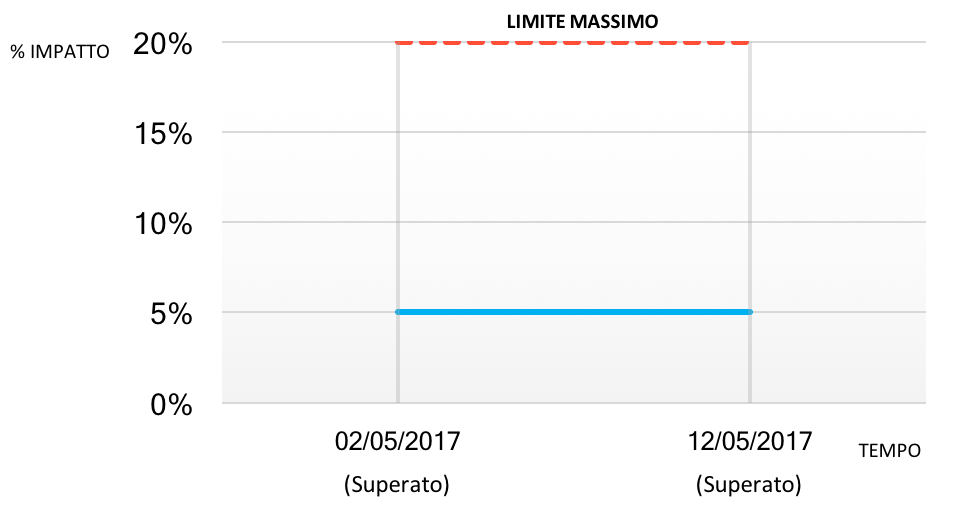
\includegraphics{grafici/Modifiche.png}
		\caption{Impatto delle modifiche - RA}
		\label{fig:modifiche}
	\end{figure}\mbox{}\\

	\begin{longtable}[c] { >{\centering\arraybackslash}p{3cm} >{\centering\arraybackslash}p{3cm} }
		\toprule
				\textbf{Valore} & \textbf{Esito} \\
			\midrule
				5\% & Superato \\
			\bottomrule
		\caption{Impatto delle modifiche - RA}
	\end{longtable}\mbox{}\\

	\newpage
	\textbf{Versioni dei browser supportate}
	\begin{figure}[!h]
		\centering
		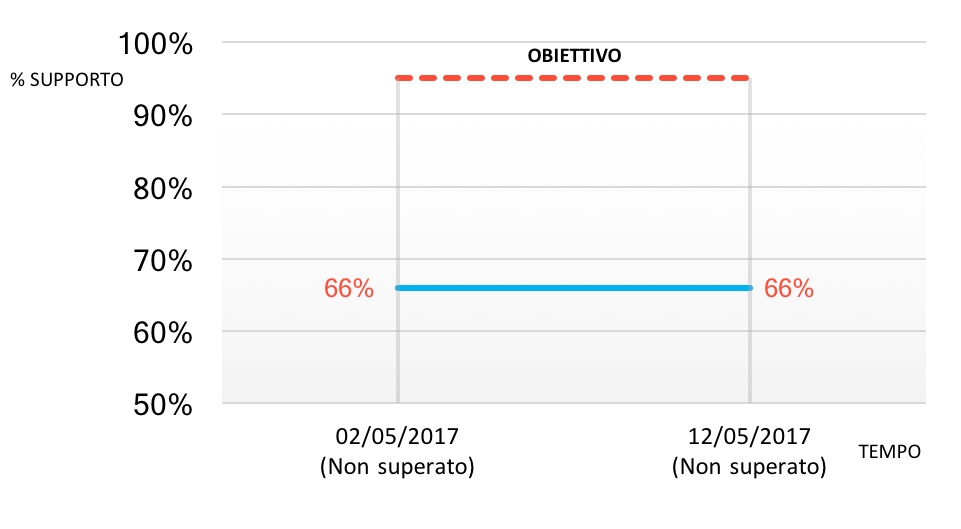
\includegraphics{grafici/Browser.png}
		\caption{Versioni dei browser supportate - RA}
		\label{fig:browser}
	\end{figure}\mbox{}\\

	\begin{longtable}[c] { >{\centering\arraybackslash}p{3cm} >{\centering\arraybackslash}p{3cm} }
		\toprule
				\textbf{Valore} & \textbf{Esito} \\
			\midrule
				66\% & Non superato \\
			\bottomrule
		\caption{Versioni dei browser supportate - RA}
	\end{longtable}\mbox{}\\

	\newpage
	\textbf{Inclusione di funzionalità da altri prodotti}
	\begin{figure}[!h]
		\centering
		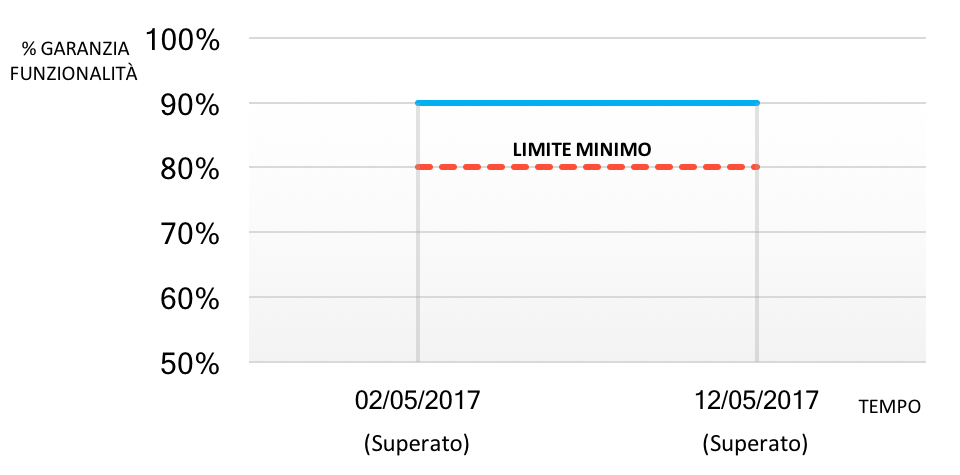
\includegraphics{grafici/Funzionalita.png}
		\caption{Inclusione di funzionalità da altri prodotti - RA}
		\label{fig:inclusione}
	\end{figure}\mbox{}\\

	\begin{longtable}[c] { >{\centering\arraybackslash}p{3cm} >{\centering\arraybackslash}p{3cm} }
		\toprule
				\textbf{Valore} & \textbf{Esito} \\
			\midrule
				90\% & Superato \\
			\bottomrule
		\caption{Inclusione di funzionalità da altri prodotti - RA}
	\end{longtable}\mbox{}\\

\end{document}
